\section{The Solenoid and the Steel Return Yoke}
\label{sec:solenoid}

The Compact Muon \emph{Solenoid} sports one of the world's most energetic solenoids, which is absolutely indispensable to the success of CMS.
It is a huge 6 meter-tall and 13 meter-long cylindrical magnet that generates a uniform magnetic field parallel to the beam line.
% the direction in which the protons collide, which we call the z direction.
When charged particles travel through this volume a Lorentz force is applied to them,
thereby separating out the particle tracks as they fly away from the IP.
% As the charged particles bend out and away from the beam pipe, they pass through the silicon tracking system, which has excellent resolution ""
% Imagine CMS as a giant camera that takes a picture every few ns of the outgoing particles. 
An enormous current of 18,000 A travels through superconducting Nb-Ti coils to produce the uniform 3.8 T magnetic field inside the volume of the solenoid (approximately 360 m$^3$)
 (Fig.~\ref{fig:cms_magnetic_field}).
%%%%%%%%%%%%%%%%%%%%
\begin{figure}[pbth]
\centering
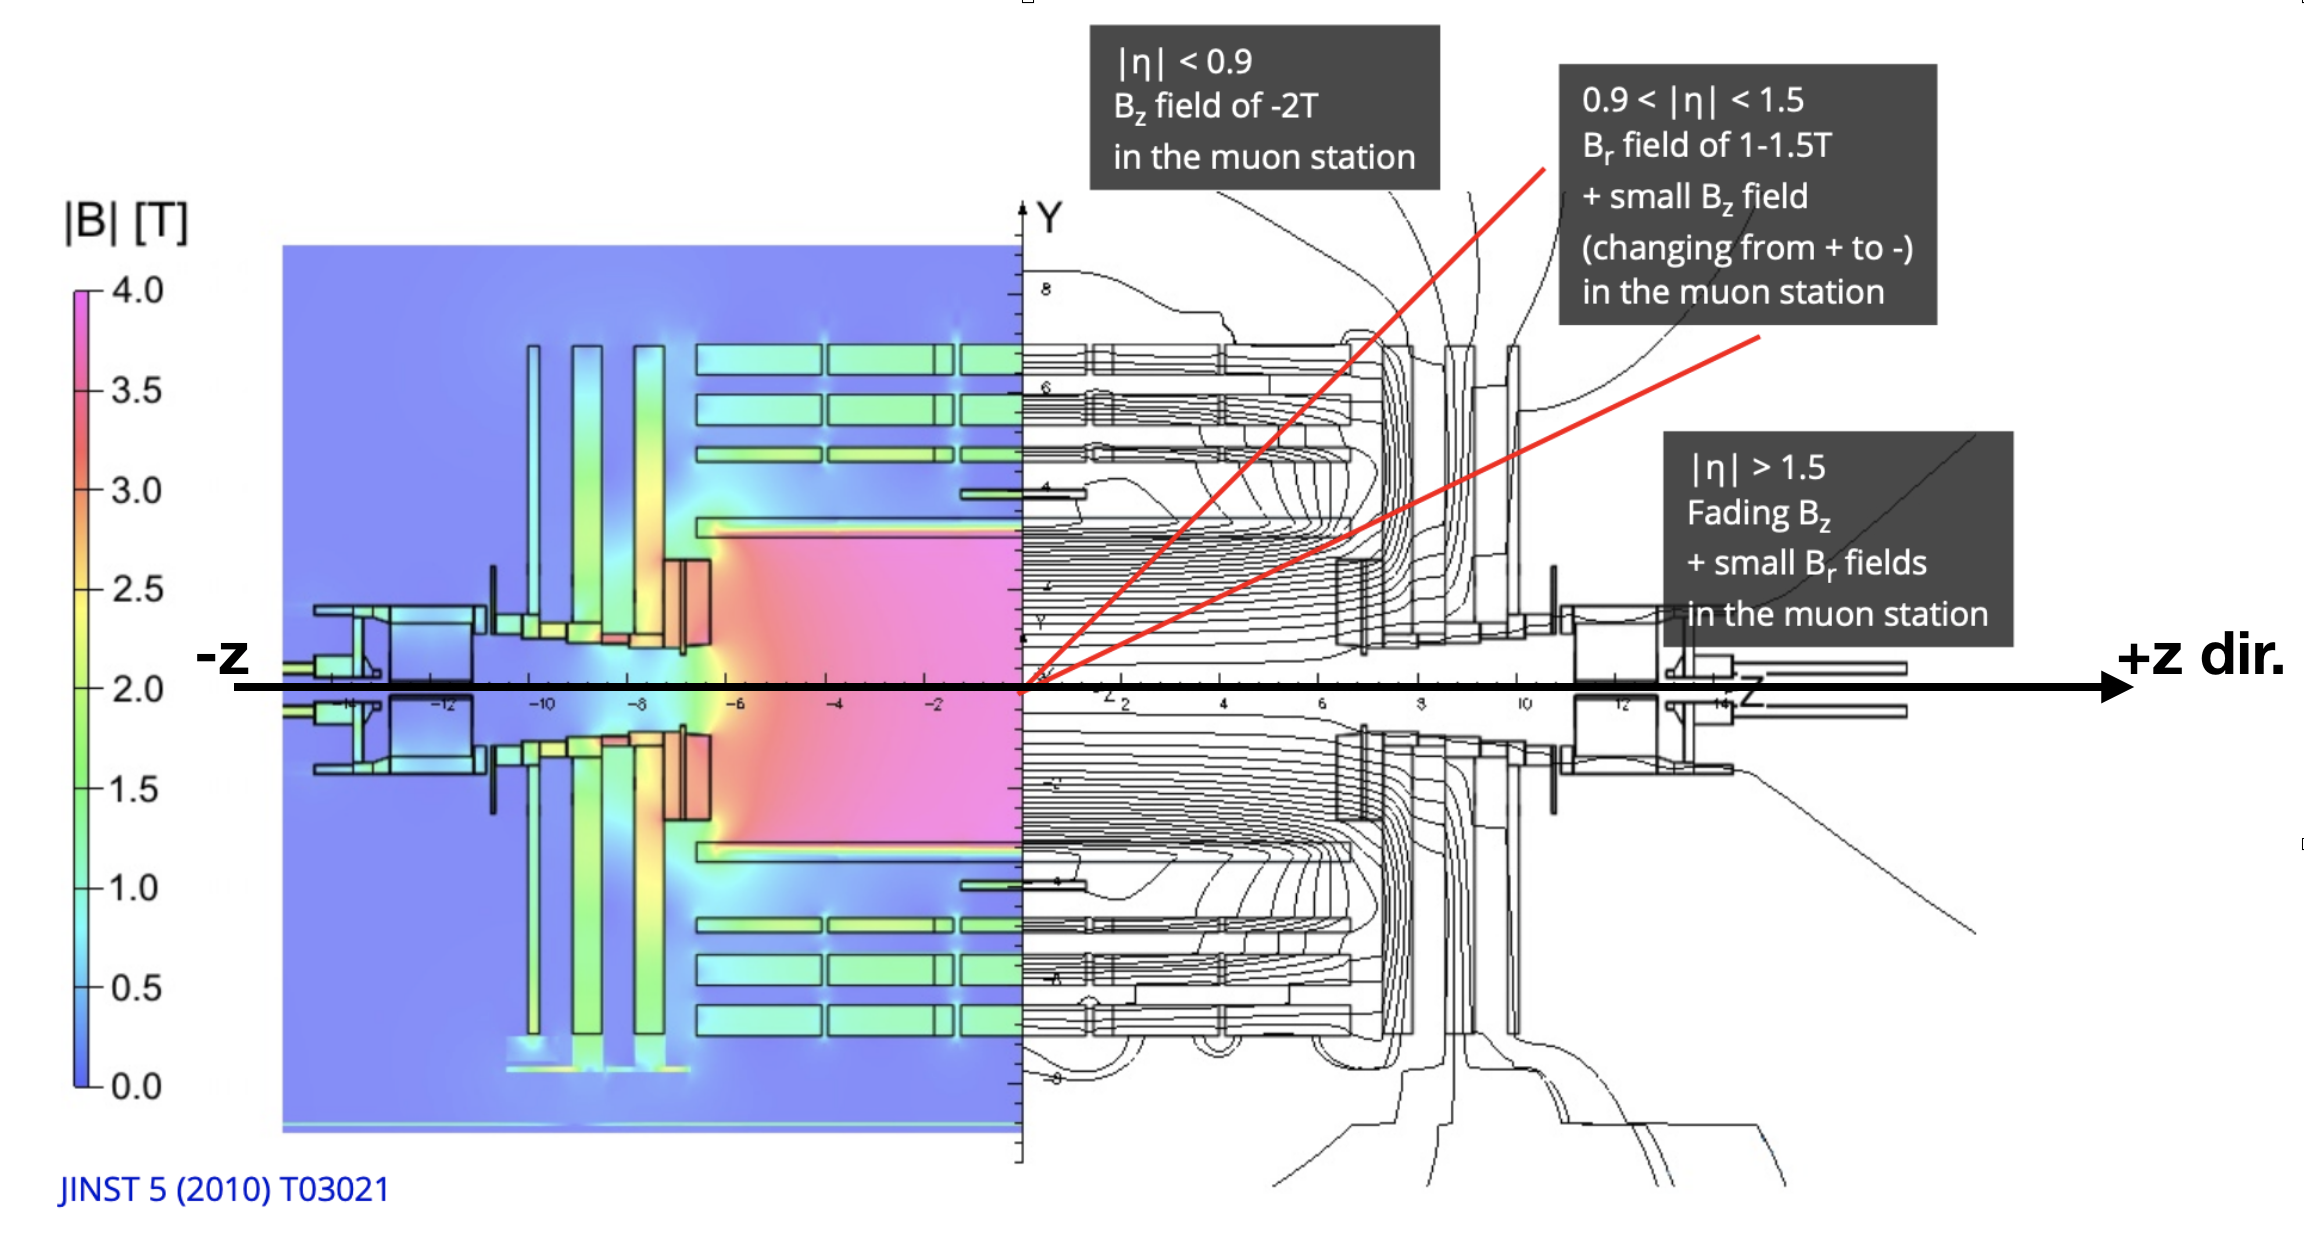
\includegraphics[width=15cm,height=15cm,keepaspectratio]{Figures/CMS_longitudinal_view_magnetic_field.png}
    \caption{
    A longitudinal cross section of CMS showing the values of the magnetic field over the volume of CMS and various field lines. 
    The magnetic field reaches its maximum of 3.8 T in the center of the detector.}
    \label{fig:cms_magnetic_field}
\end{figure}
%%%%%%%%%%%%%%%%%%%%
This magnetic field is 100,000 times stronger than the Earth's magnetic field.
A massive 2.7 GJ of energy is stored in the magnetic field of CMS. 
This is about the same amount of energy found in an Airbus A320 in flight!

{\bf Steel Return Yoke:} 
Most of the mass of CMS comes from the steel return yoke which helps to redirect the powerful magnetic field back on itself. 
The yoke system constitutes 12,500 tonnes, which is 89\% of CMS's total mass.

% \section{Electronics?}
%%%%%%%%%%%%%%%%%%%%
\begin{figure}[pbth]
\centering
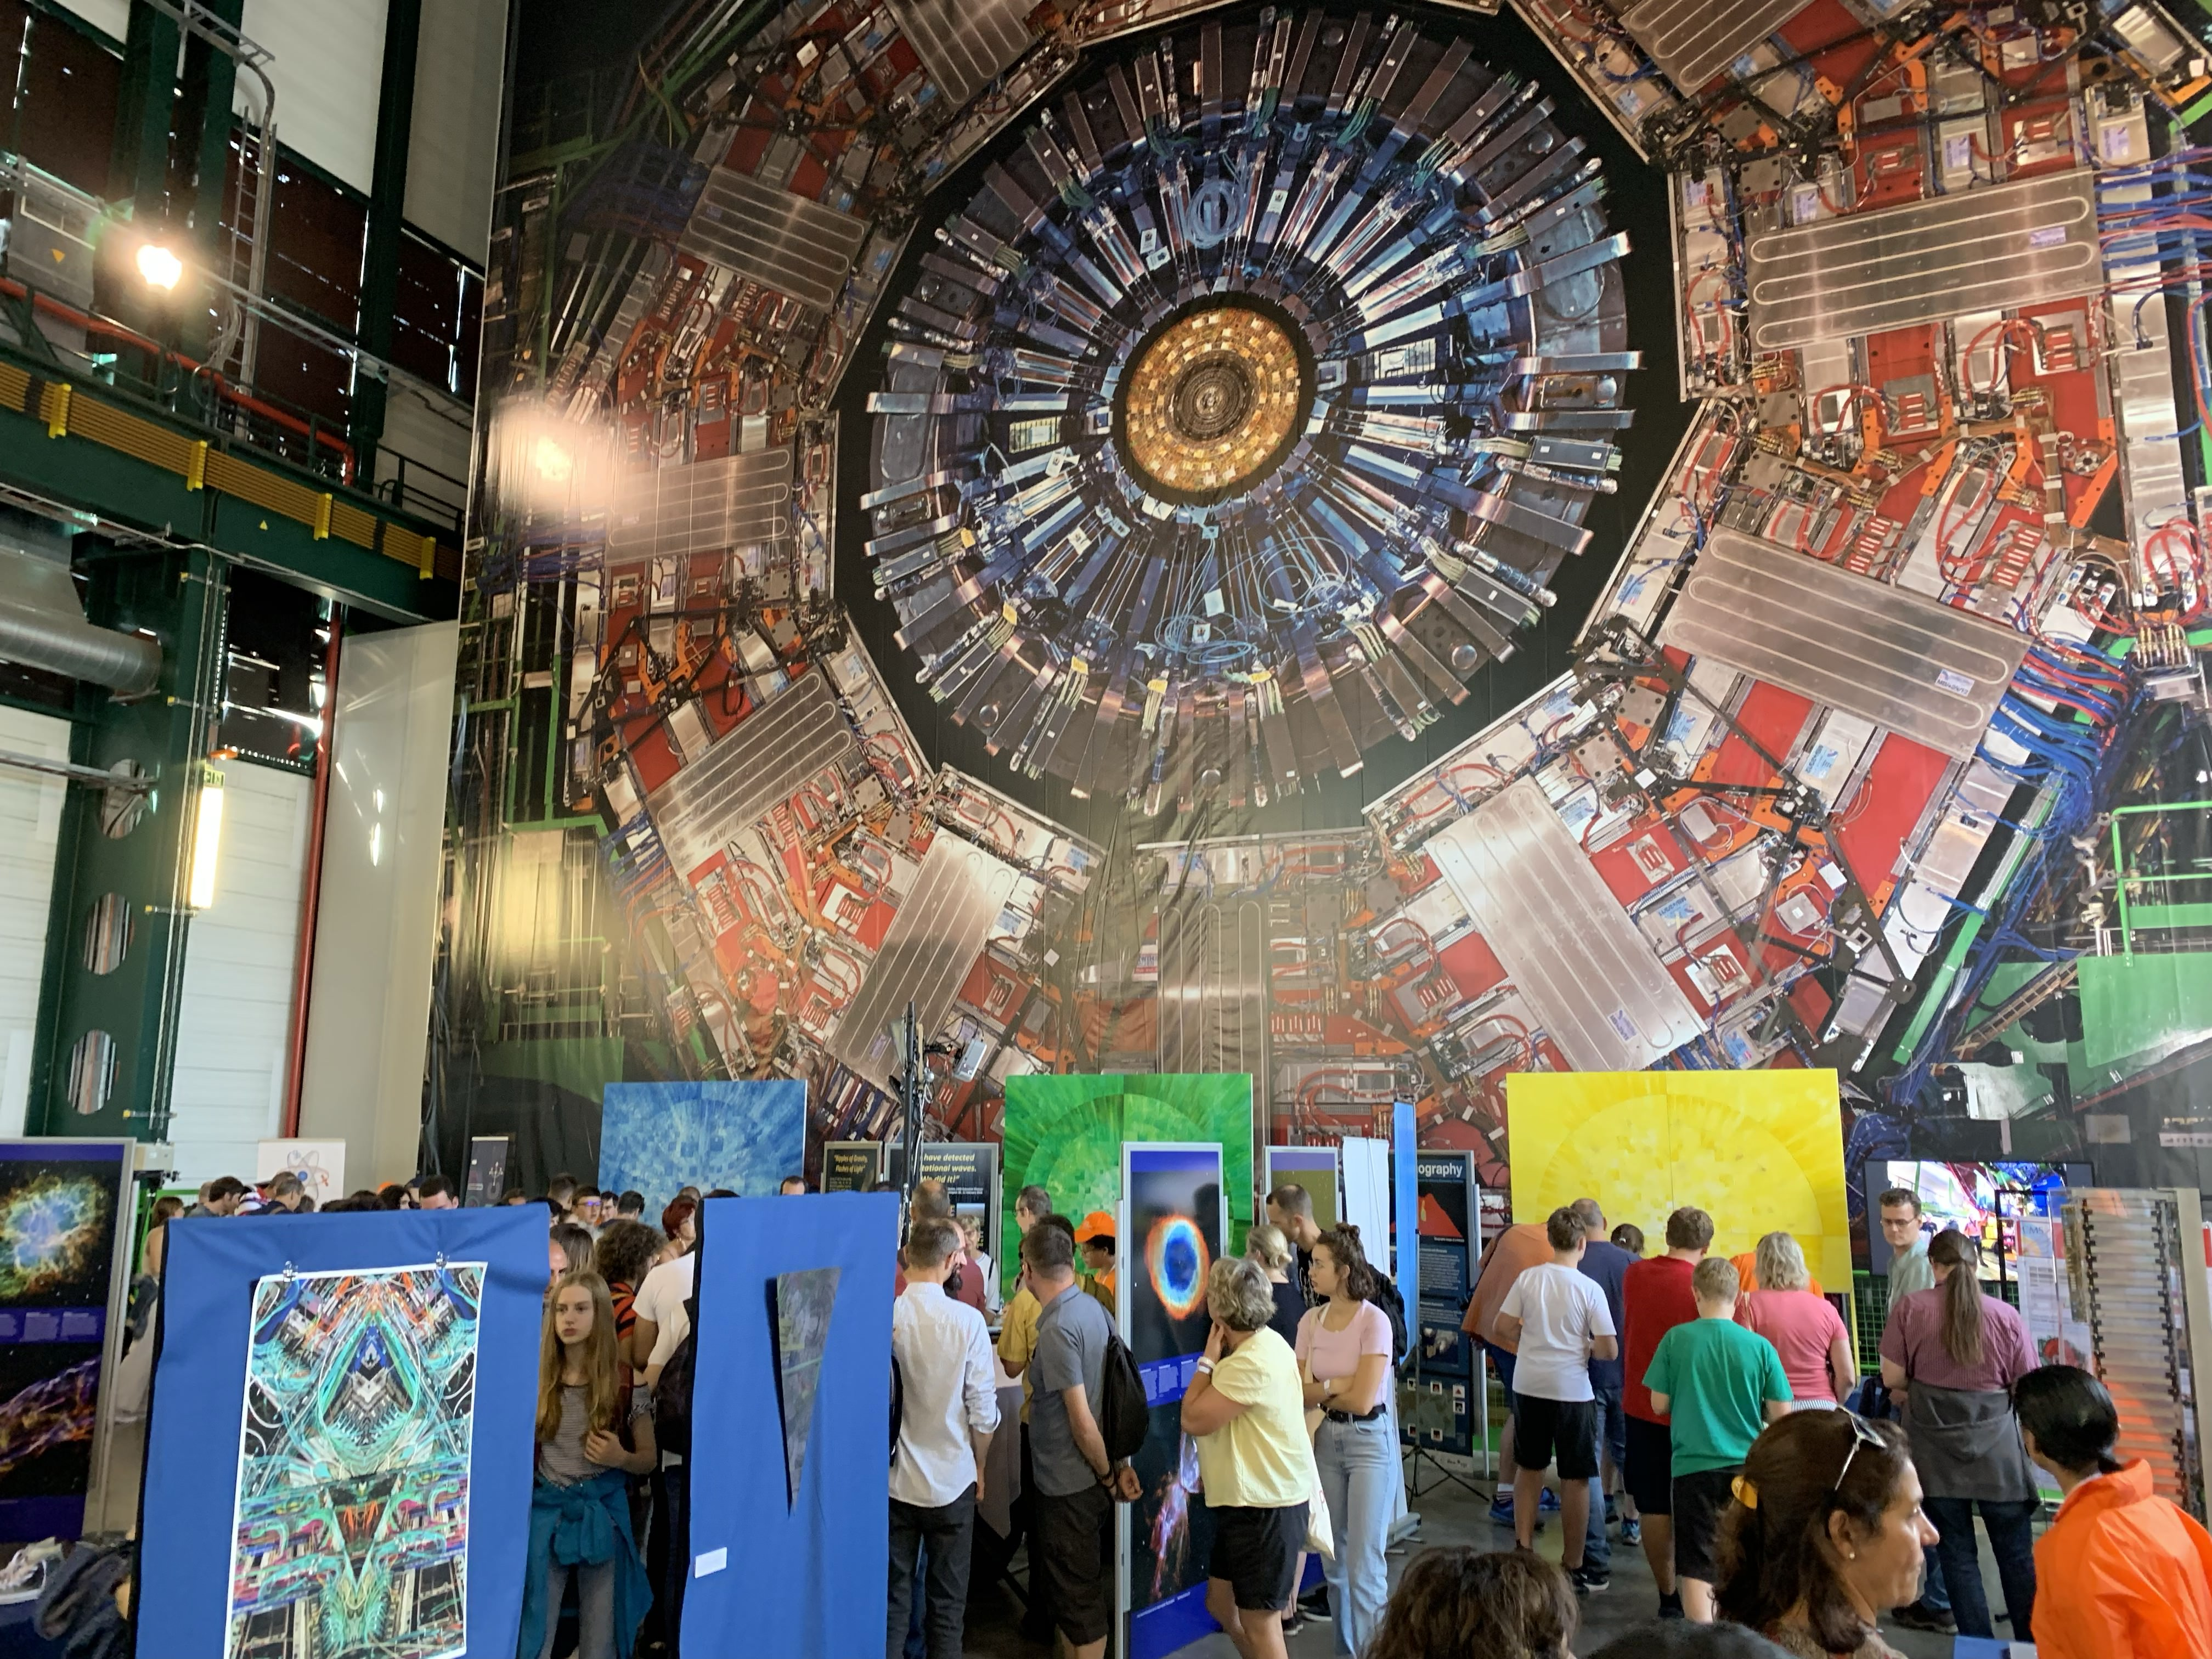
\includegraphics[width=10cm,height=10cm,keepaspectratio]{Figures/CMS_poster_SX5.jpg}
    \caption{
    Life-size poster of the CMS detector, taken during CERN Open Days 2019
    in the SX5 warehouse where parts of CMS were assembled.}
    \label{fig:cms_poster}
\end{figure}
%%%%%%%%%%%%%%%%%%%%
Weighing in at a whopping 14,000 tonnes, 
standing 5 stories tall (15 meters, see Fig.~\ref{fig:cms_poster}), and reaching 29 meters long, 
the Compact Muon Solenoid (CMS) is a ``general-purpose detector'' situated at Point 5 along the LHC (Fig.~\ref{fig:lhc_points}).
The purpose of CMS is to detect many of the decay products 
that come out from the $pp$ collisions to be used for analyses.
%%%%%%%%%%%%%%%%%%%%
\begin{figure}[pbth]
\centering
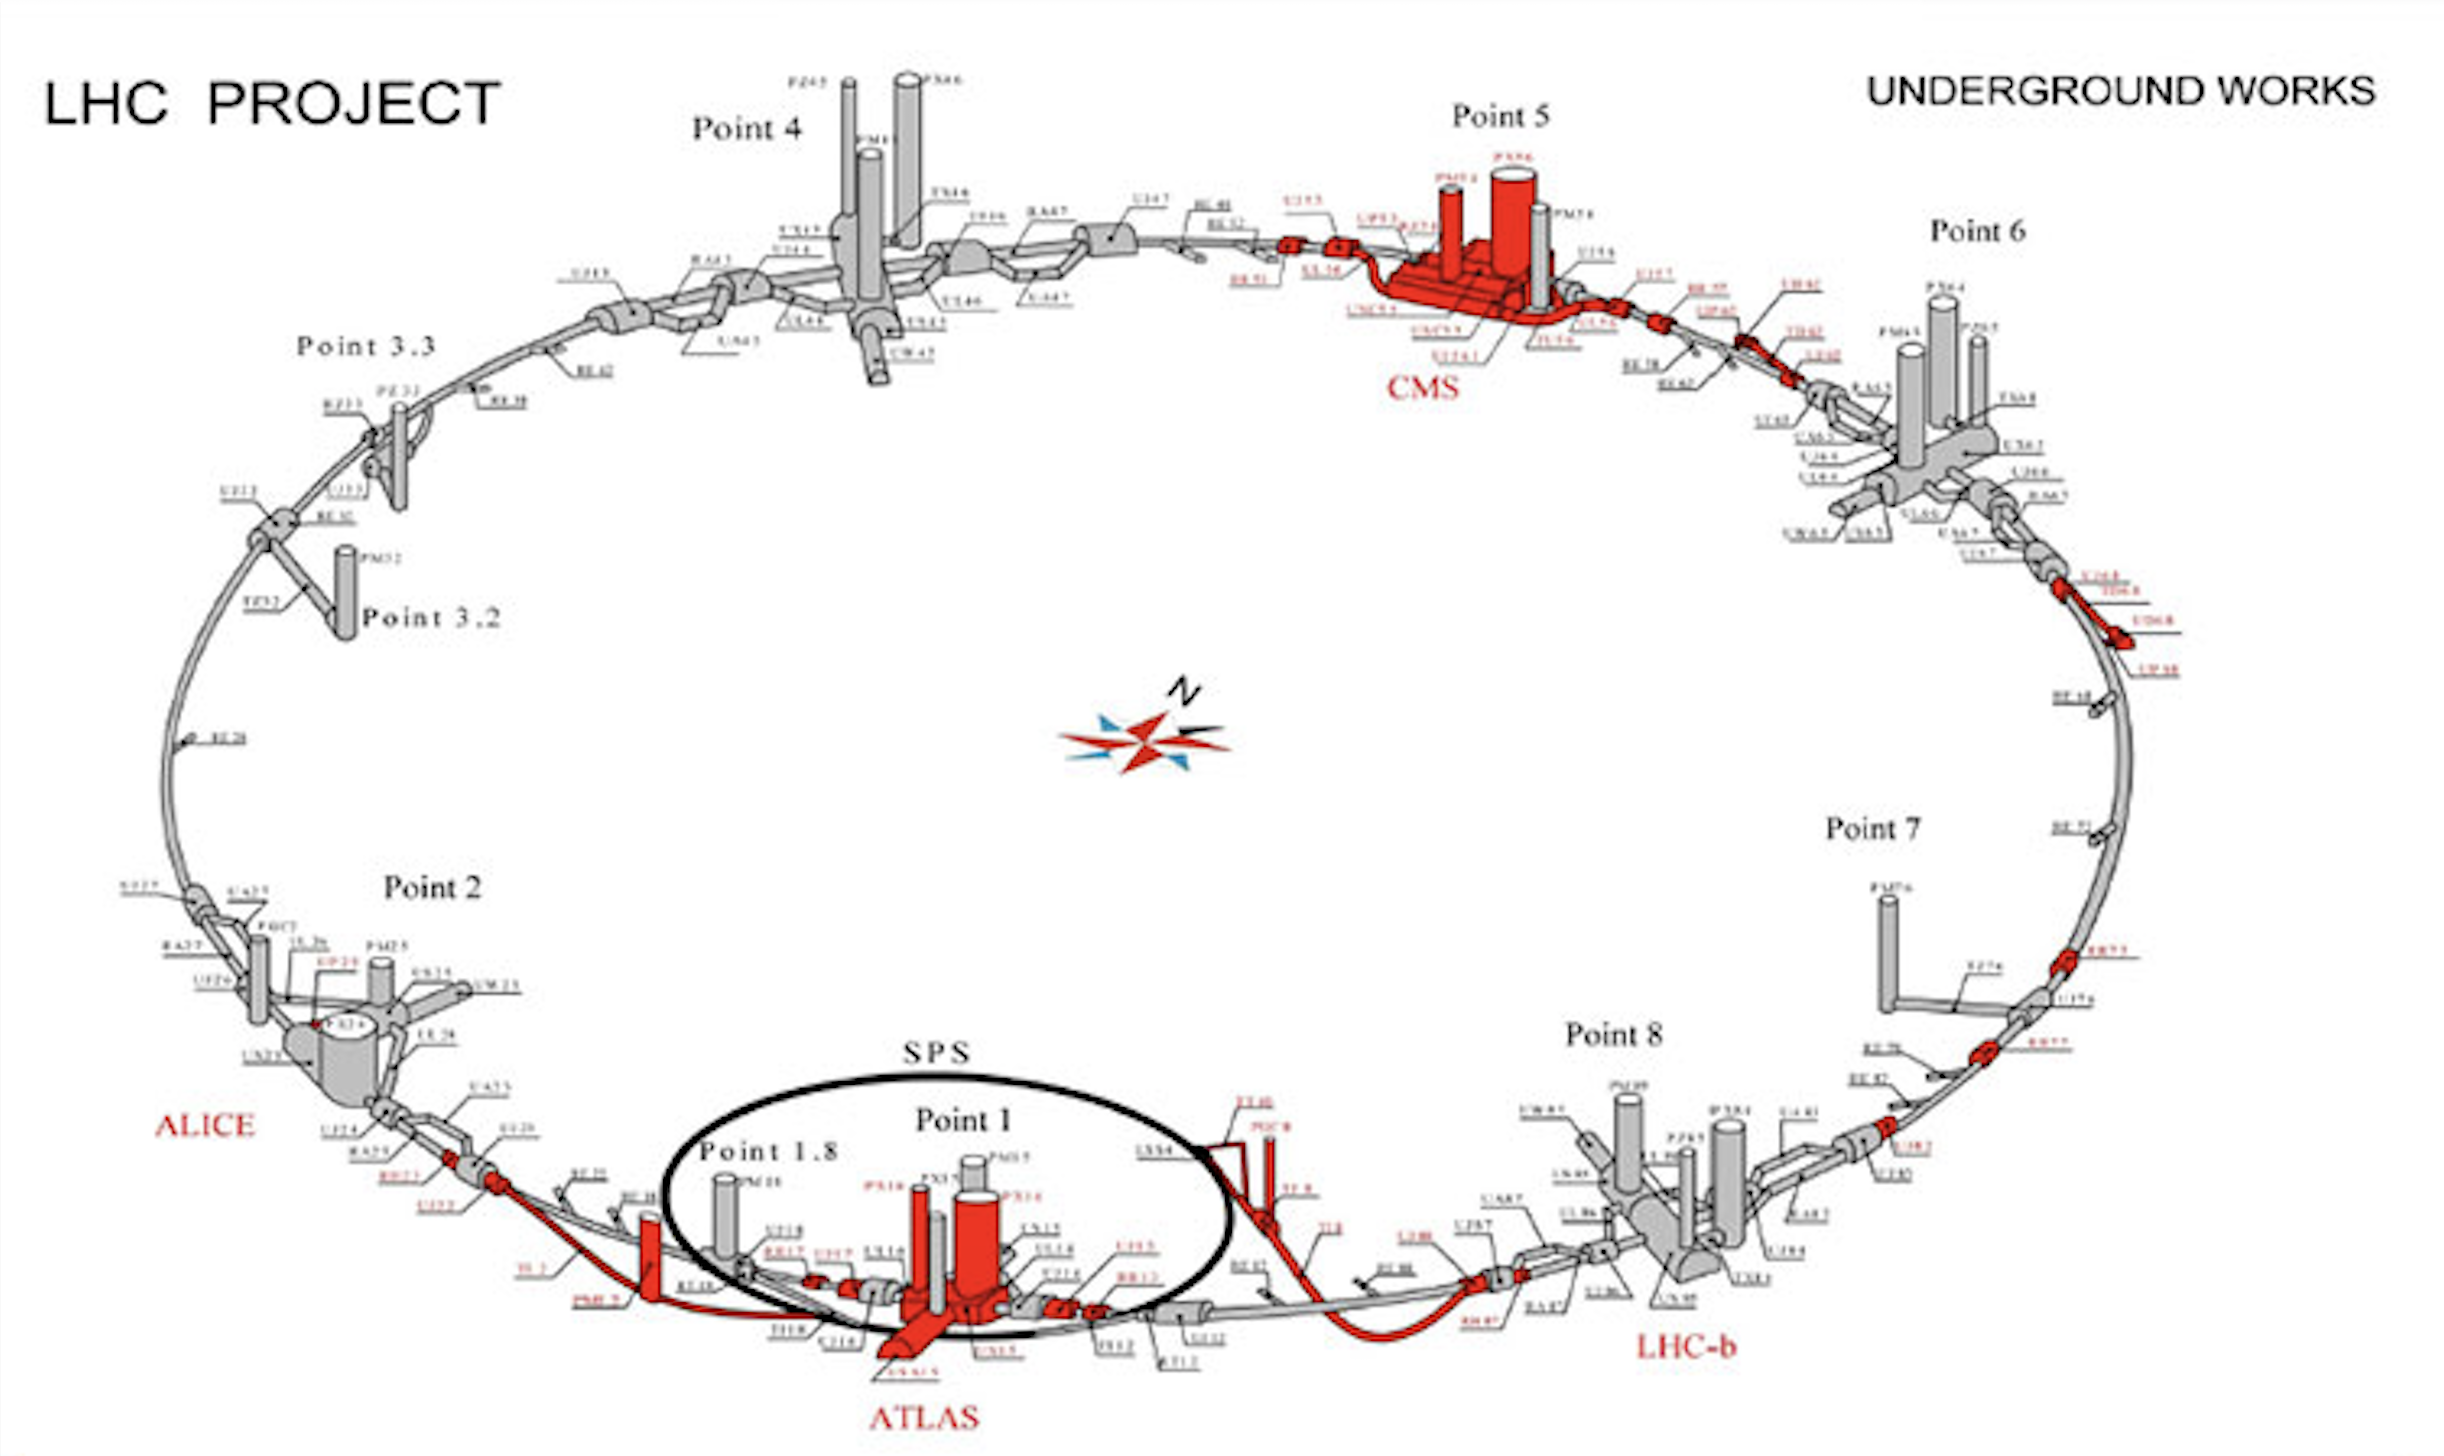
\includegraphics[width=13cm,height=13cm,keepaspectratio]{Figures/lhc_points_with_buildings.png}
    \caption{
    Points 1 through 8 along the LHC.
    Collisions occur at 
    Points 1 (ATLAS), 2 (ALICE), 5 (CMS), and 8 (LHCb),
    whereas the remaining points are used for LHC beam maintenance and testing.} 
    \label{fig:lhc_points}
\end{figure}
%%%%%%%%%%%%%%%%%%%%
CMS is composed of a series of concentric subdetectors that filter the outgoing particles in a clever way (Fig.~\ref{fig:cms_cut_out_view}).
%%%%%%%%%%%%%%%%%%%%
\begin{figure}[pbth]
\centering
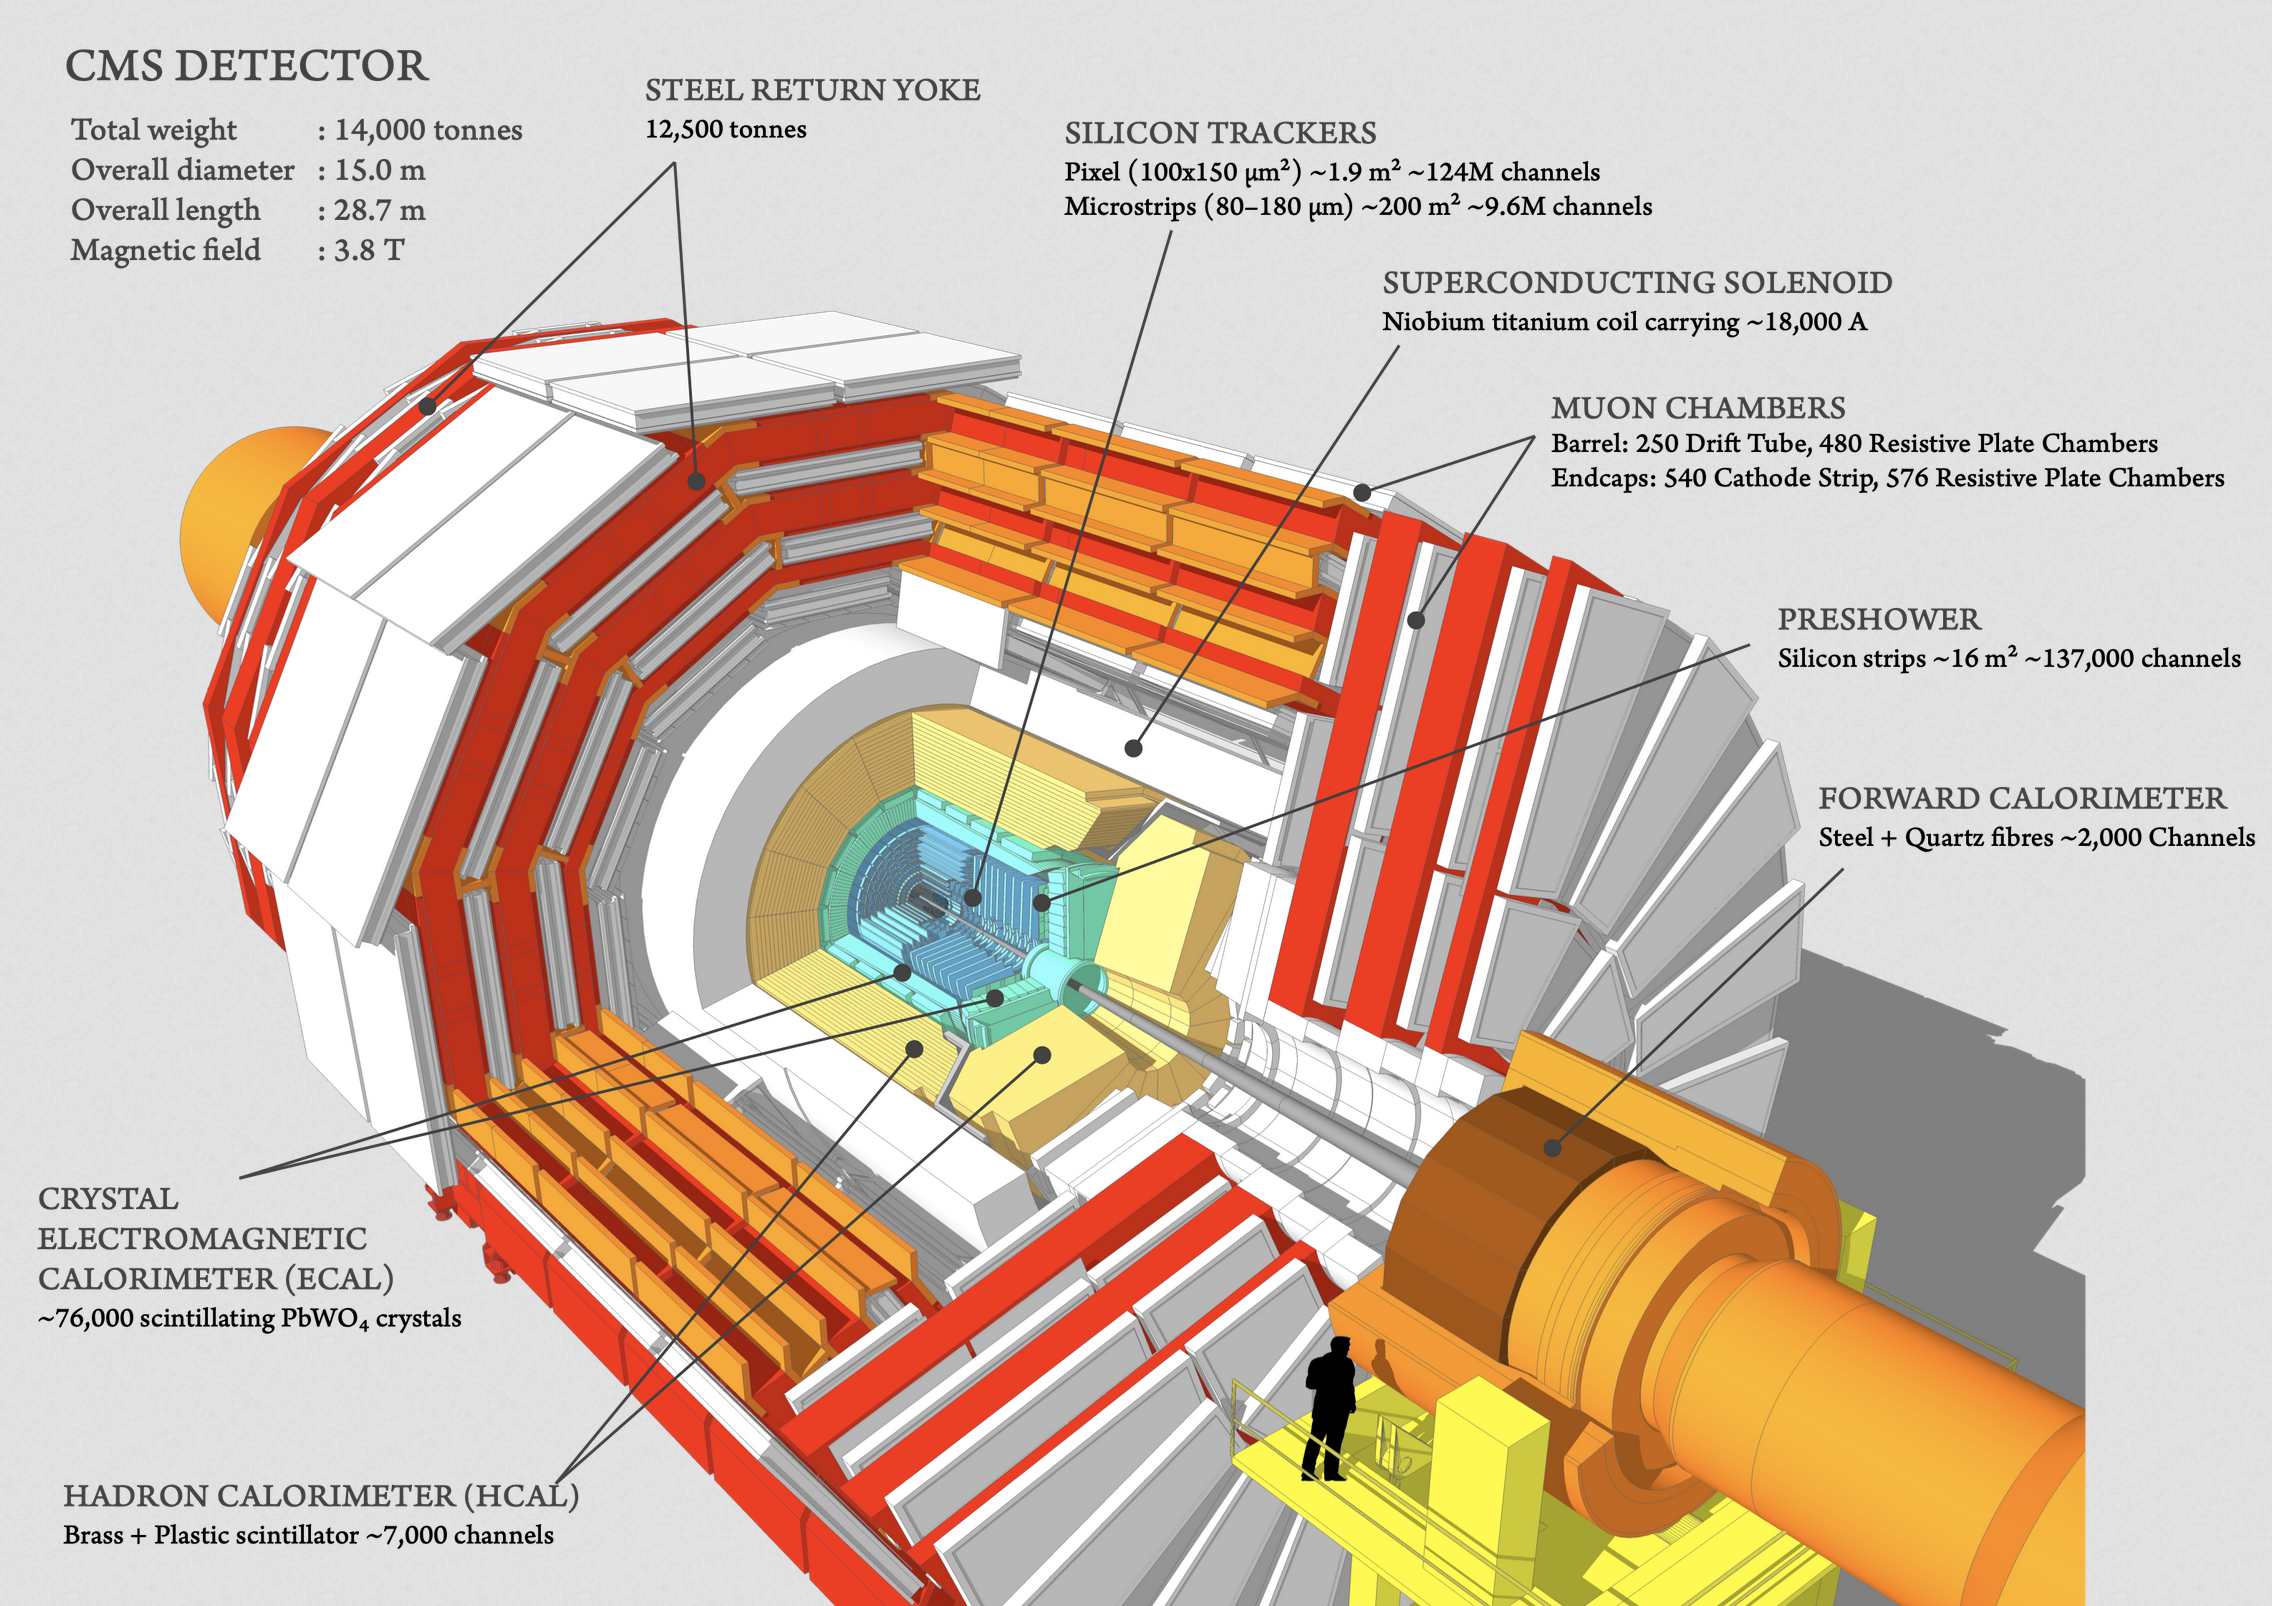
\includegraphics[width=15cm,height=15cm,keepaspectratio]{Figures/CMS_cut_away.png}
    \caption{Cut out of the CMS detector showing its various subdetector components.} 
    \label{fig:cms_cut_out_view}
\end{figure}
%%%%%%%%%%%%%%%%%%%%
Depending on which subdetector, or combination of subdetectors were hit by the outgoing particles, the type of particle can be deduced and its energy, momentum, and trajectory are measured too.
A few example particles and their associated tracks are shown in Fig.~\ref{fig:cms_particle_trajectories}. 

In the sections below, I describe the various subdetectors which surround the interaction point (IP), the point where the $pp$ collision occurs in the beam pipe.
%%%%%%%%%%%%%%%%%%%%
\begin{figure}[pbth]
\centering
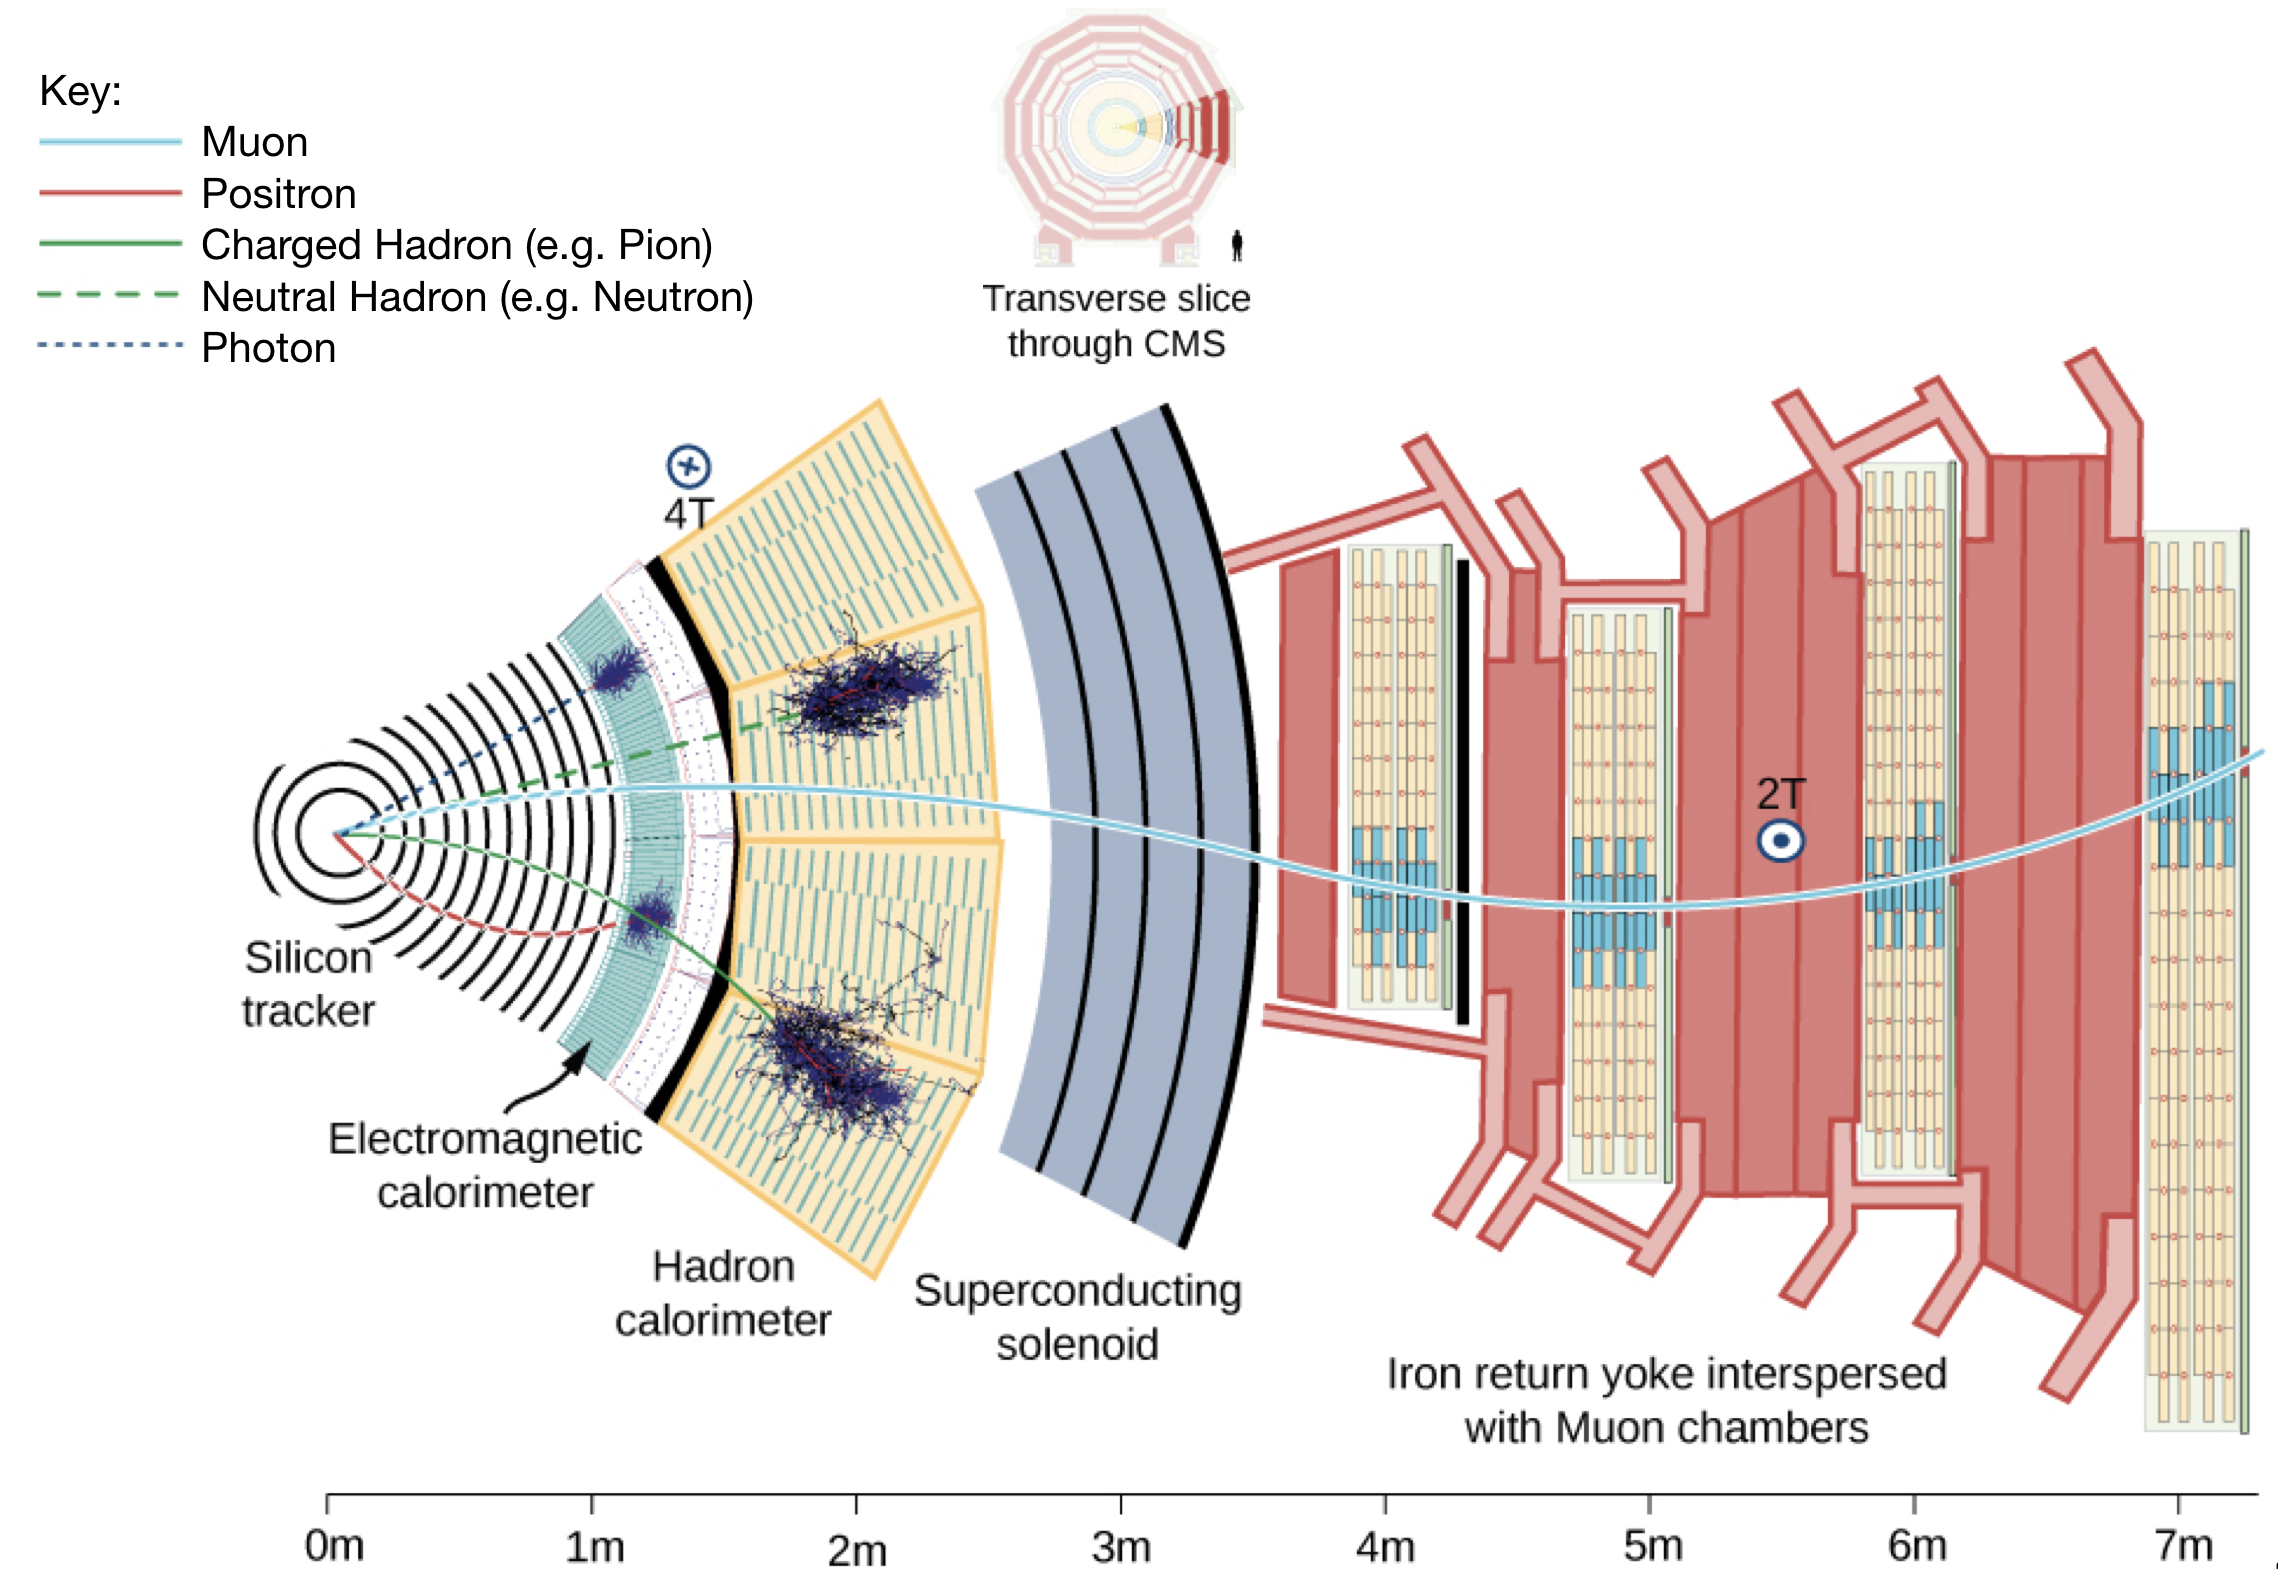
\includegraphics[width=15cm,height=15cm,keepaspectratio]{Figures/CMS_transverse_particletrajectories_corrected.png}
    \caption{
    A transverse view of CMS showing the ``filtration process'' as different particles pass through different subdetectors.
    A positron (solid red line) curves due to the presence of the magnetic field and gets stopped in the ECAL, creating an EM shower.
    A photon (blue dashed line) does not get detected at all by the Silicon Tracker, since it has no electric charge.
    It continues through to the ECAL and makes a shower here, like the positron.
    Charged hadrons (solid green line) will show curved tracks from the Silicon Tracker, may leave some trace in the ECAL, but primarily get stopped by the HCAL creating hadronic showers.
    Neutral hadrons (dashed green line) do not interact with the tracker, and only undergo EM showers a little in the ECAL, but show most energy deposits in the HCAL.
    Muons (solid blue line) are detected by the Silicon Tracker and then mostly pass through the other subdetectors without interacting until they finally reach the Muon System.
    % In fact you can even determine whether its charge is positive or negative since
    % q v cross B gives the direction of Force.
    % The velocity of the muon is out like this, and the B field is into the screen, so the applied force would be up like this for a positive particle. 
    Using the Lorentz force law and knowing which direction the magnetic field is pointing (Section~\ref{sec:solenoid}), one can deduce the sign of the charge of the particle. 
    Based on the radius of curvature from the trajectory, one can then calculate the momentum and energy of the particle.
    % We see that it's not curving up, but curving the other way so we know it must be negative.
    % Notice that since it is curving the opposite way from the muon so we know this is a positive particle.
    % Next up the solid green trajectory represents a charged hadron, like for example maybe an antiproton that got produced.
    % Notice that it would be the same sign as the muon because they curve in the same direction.
    } 
    \label{fig:cms_particle_trajectories}
\end{figure}
%%%%%%%%%%%%%%%%%%%%
% After the protons collide, they make a mess of all sorts of particles:
% electrons, lambda baryons, kaons, muons, photons...

%%%%%%%%%%%%%%%%%%%%%%%%%%%%%
%----- Silicon Tracker -----%
%%%%%%%%%%%%%%%%%%%%%%%%%%%%%
\section{Silicon Tracker}
CMS is home to one of the world's largest silicon detectors, the so-called {\bf Silicon Tracker}.
The main purpose of the Tracker is to, well... \emph{track} the trajectories very precisely of outgoing particles from the IP.
It consists of two types of pure silicon detectors: the pixel detector and the strip detector, each of which is described next: 
% , and are absolutely necessary to \emph{track} the decay products from $pp$ collisions.

{\bf Pixel Detector:} The inner part, the closest subdetector of CMS to the IP, is the pixel detector made of minuscule silicon ``pixels'', as shown in Fig.~\ref{fig:tracker_real} (Left, pink).
Each pixel is 100$\mu$m x 150$\mu$m in size and, with 66 million of them, they altogether cover a sensitive area of 1.9 m$^2$. 
The pixel detector has the highest particle flux out of any other subdetector, since it sits only 8 cm away from the beam pipe:
it receives around 10 million particles per cm$^2$ per second.
The pixel detector is made of three cylindrical layers and two endcaps that surround the beam pipe.
Impressively, the pixel detector has around 6,000 connections (channels) per cm$^2$.

{\bf Strip Detector:} The second and outer part of the Silicon Tracker is called the strip detector, which has 10 million detector strips spread across 10 cylindrical layers.
The first 4 layers belong to the tracker inner barrel (TIB) and the remaining 6 layers belong to the tracker outer barrel (TOB), Fig.~\ref{fig:tracker_real} (Left, green and blue, respectively). 
Both the TIB and TOB have two endcaps associated with them, the TID and TEC, respectively.
Accounting for all of its components, the strip detector is sensitive to 200 m$^2$.
Fig.~\ref{fig:tracker_xs} gives a clearly-labelled transverse illustration of the pixel and strip detectors.
% It functions similarly to the pixels in that 
% It also has has slightly worse resolution than the pixel detector.
% Both the pixel and strip trackers have barrel and endcap components for nearly hermetic coverage around the beam pipe.
%%%%%%%%%%%%%%%%%%%%
\begin{figure}[pbth]
\centering
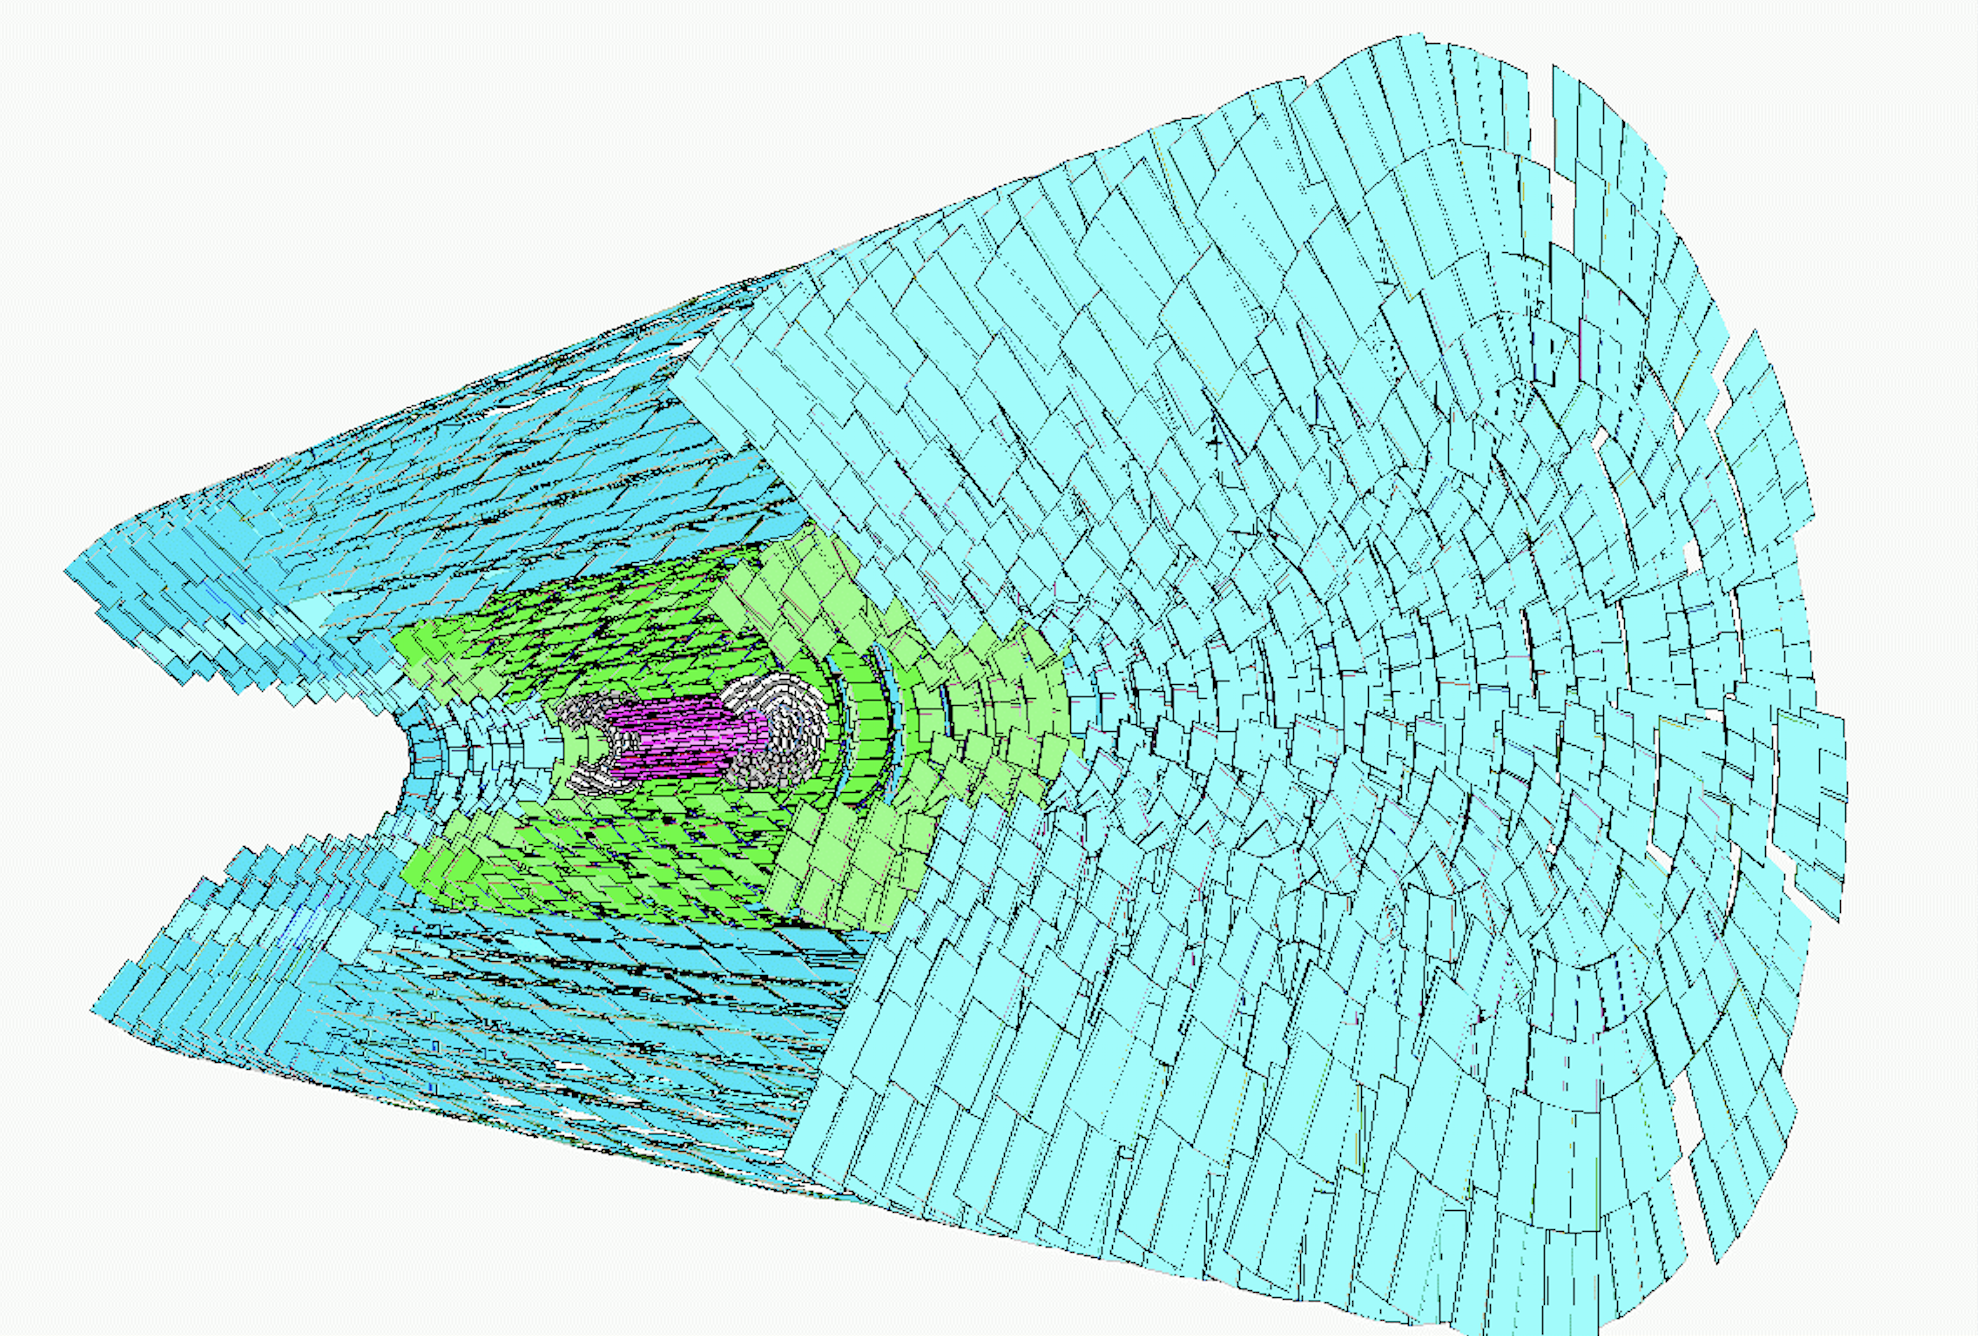
\includegraphics[width=0.49\textwidth,height=10cm,keepaspectratio]{Figures/silicon_tracker_simulated.png}
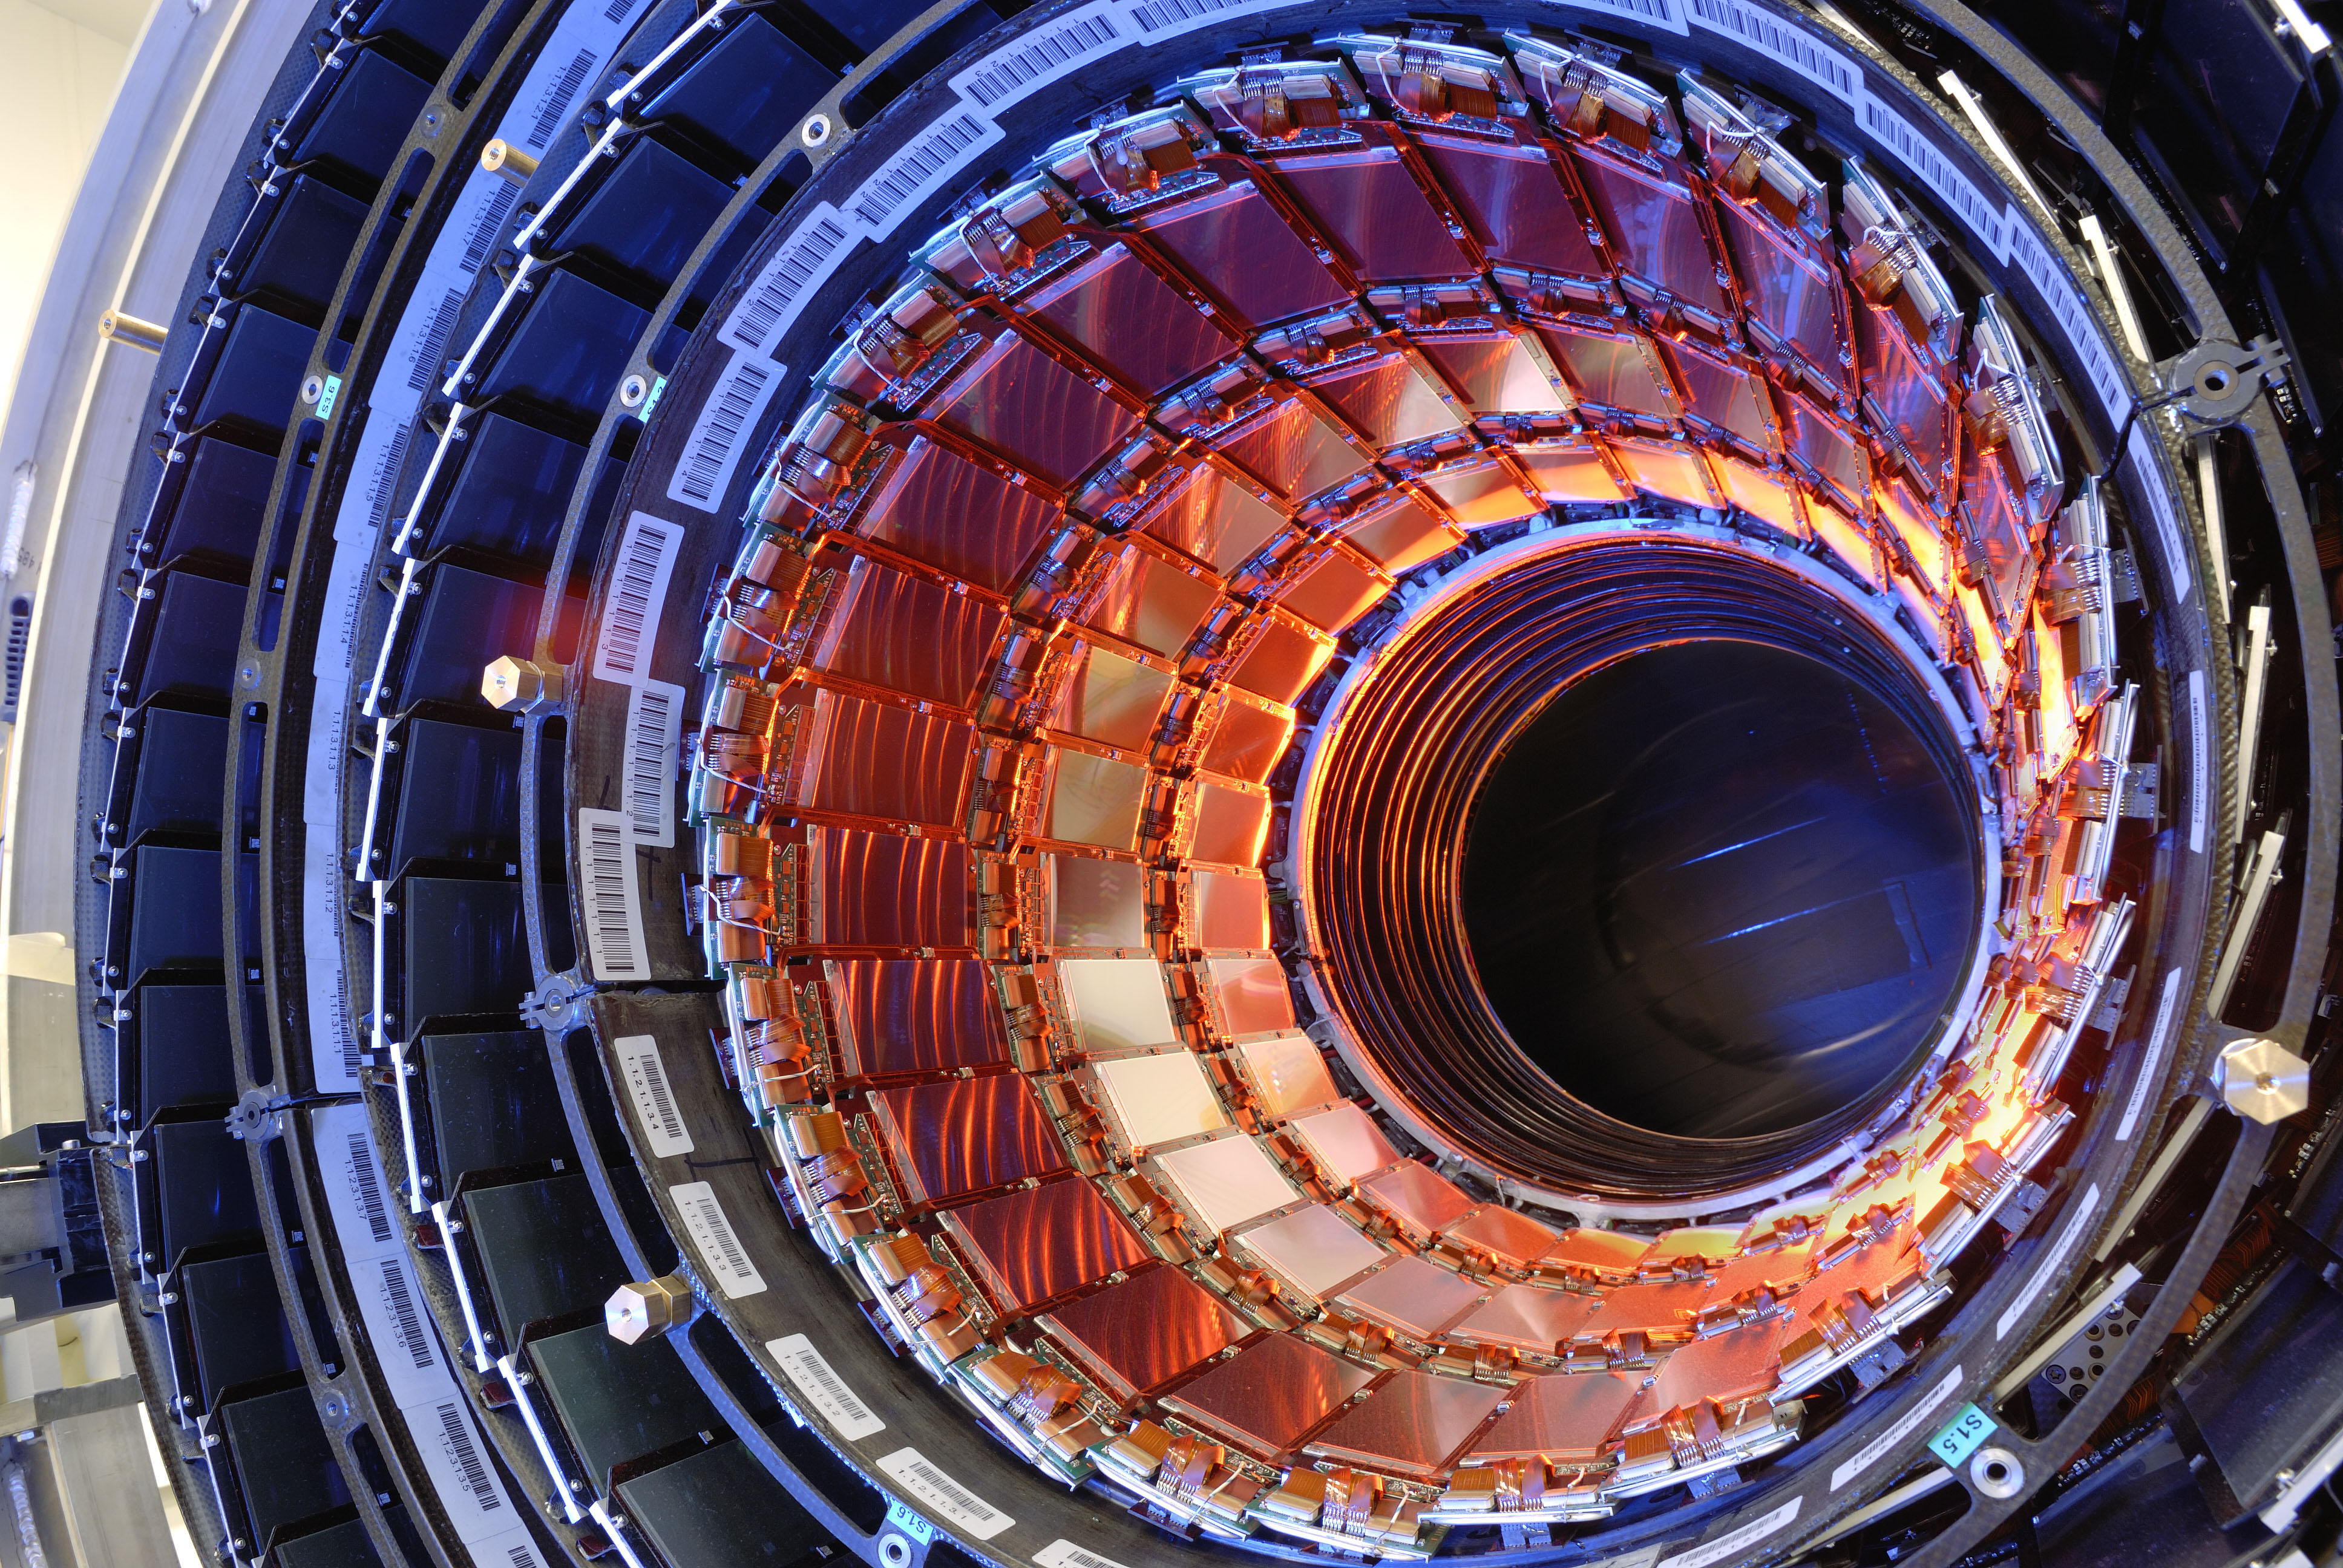
\includegraphics[width=0.49\textwidth,height=10cm,keepaspectratio]{Figures/silicon_tracker_real.jpg}
    \caption{
    (Left) A simulation of the Silicon Tracker, showing the 3 cylindrical layers of the pixel detector (pink), 4 layers of the TIB (green) and the 6 layers of the TOB (blue) of the strip detector.
    The endcap components are also shown.
    (Right) A real picture of the Silicon Tracker. Purdy, isn't it?} 
    \label{fig:tracker_real}
\end{figure}
%%%%%%%%%%%%%%%%%%%%
\begin{figure}[pbth]
\centering
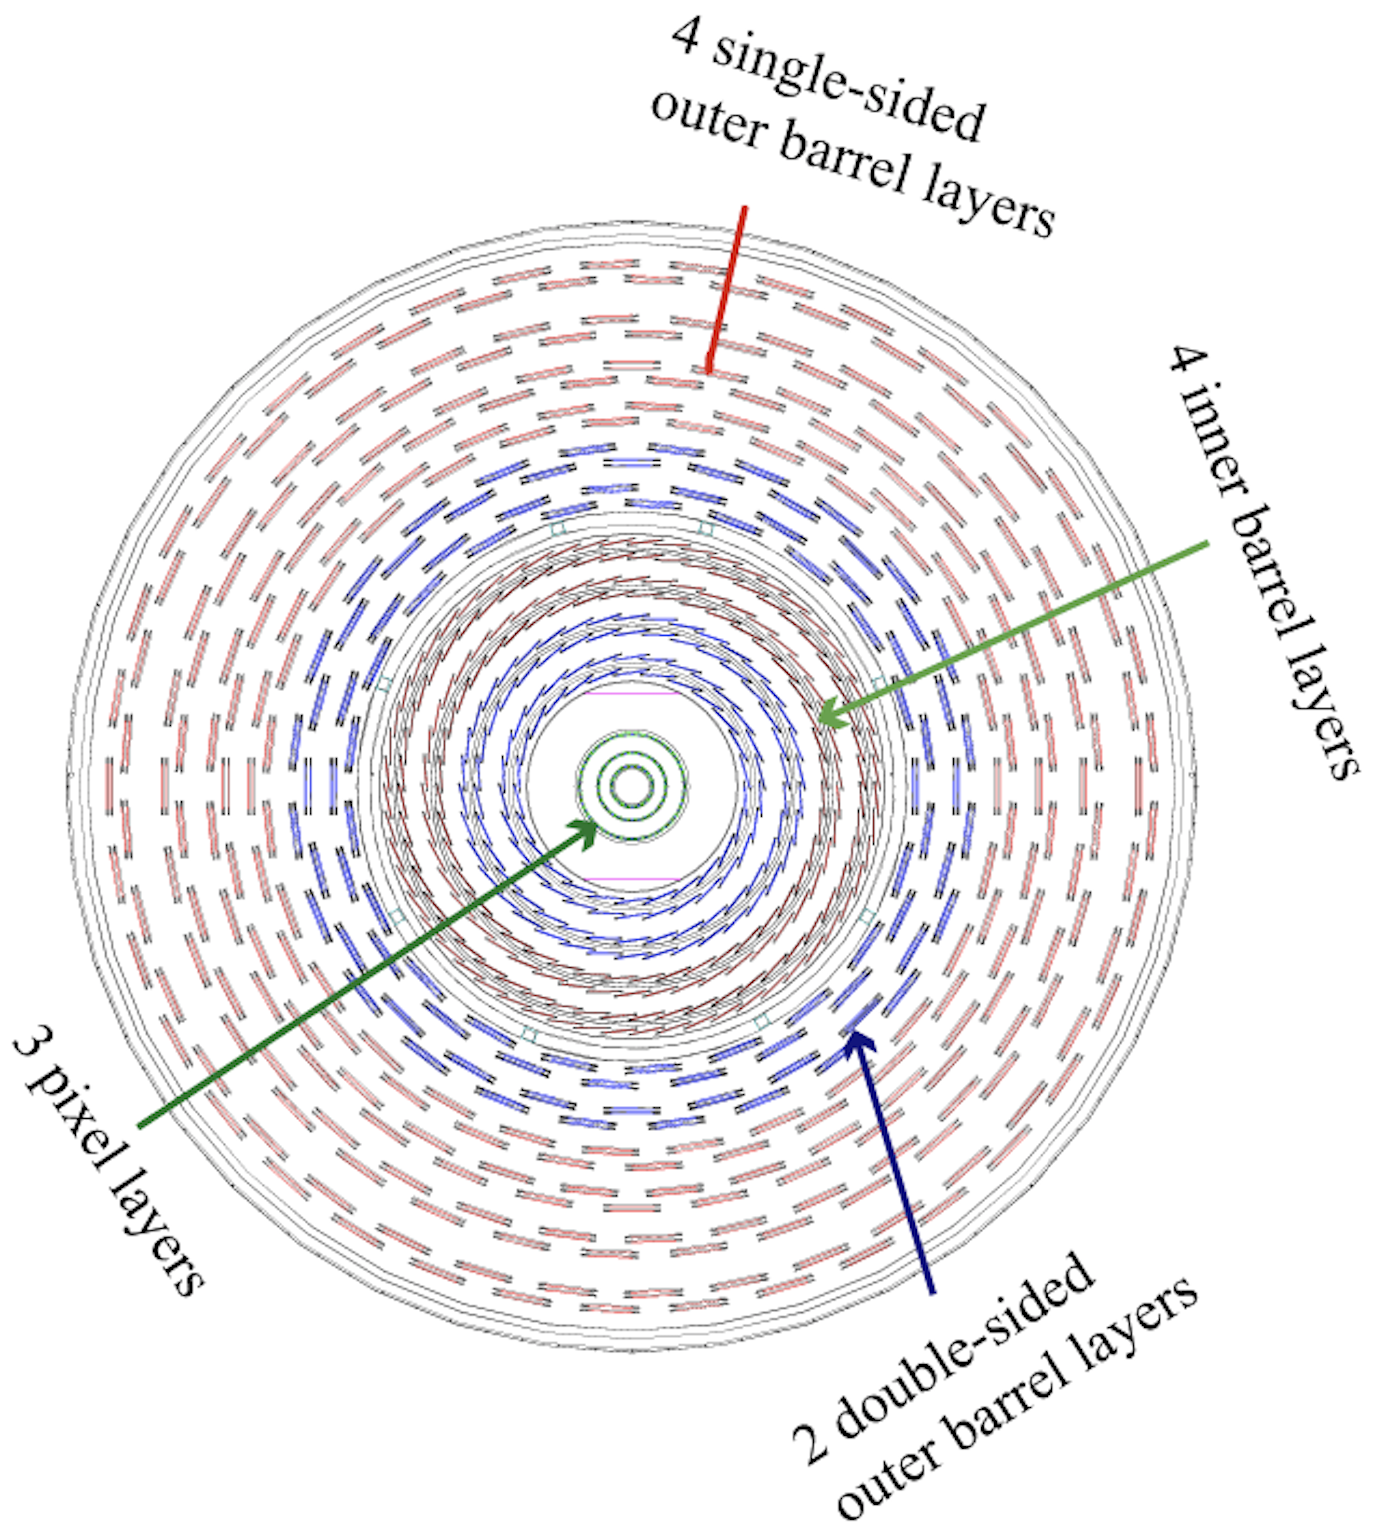
\includegraphics[width=10cm,height=10cm,keepaspectratio]{Figures/silicon_tracker_transverse_view.png}
    \caption{A transverse view of the silicon pixel and strip detectors, explicitly labelling the different layers involved.}
    \label{fig:tracker_xs}
\end{figure}
%%%%%%%%%%%%%%%%%%%%

Consider the life of a particle produced from a $pp$ collision:
Starting at the IP, the produced particles first have an opportunity to interact with the Tracker (Fig.~\ref{fig:tracker_real}, Right).
Only charged particles will generate ``hits'' in the Silicon Tracker.
Therefore, photons, neutrons, and neutral pions, \eg, are invisible to the tracker.
Given enough hits and using sophisticated reconstruction software, we can determine precisely how the particle passed through the tracker.
It's essentially a fancy game of ``connect-the-dots'' to determine the particle's trajectory.
Figuring out the trajectory allows one to measure the radius of curvature, and therefore the momentum of the particle.
This is what makes the Silicon Tracker such an important subdetector.

Another major benefit of the Silicon Tracker is its assistance in vertex identification.
During pile up (multiple proton collisions happening within the same BX),
the tracker can distinguish between proton collisions with a resolution of about 
100 $\mu$m longitudinally and 50 $\mu$m transverse to the beam pipe.
This is crucial to being able to figure out which outgoing particles came from which $pp$ vertex.
Since the tracker wasn't built to catch particles, they usually continue on to the next subsystems.
Thus, CMS must be built as a kind of ``particle filter''.
Electrons and photons are the first to be filtered out by the Electromagnetic Calorimeter...

%%%%%%%%%%%%%%%%%%
%----- ECAL -----%
%%%%%%%%%%%%%%%%%%
\section{Electromagnetic Calorimeter}
After particles pass through the Silicon Tracker system, they encounter the {\bf Electromagnetic Calorimeter} (ECAL). 
This is a scintillating subdetector made out of approximately 78,000 beautiful, transparent, and heavy ${\rm PbWO_{4}}$ crystals, as shown in Fig.~\ref{fig:ecal_crystals} (Left).
Each crystal weighs 1.5 Kg but has only the volume of a small cup of coffee. 

%%%%%%%%%%%%%%%%%%%%
\begin{figure}[pbth]
\centering
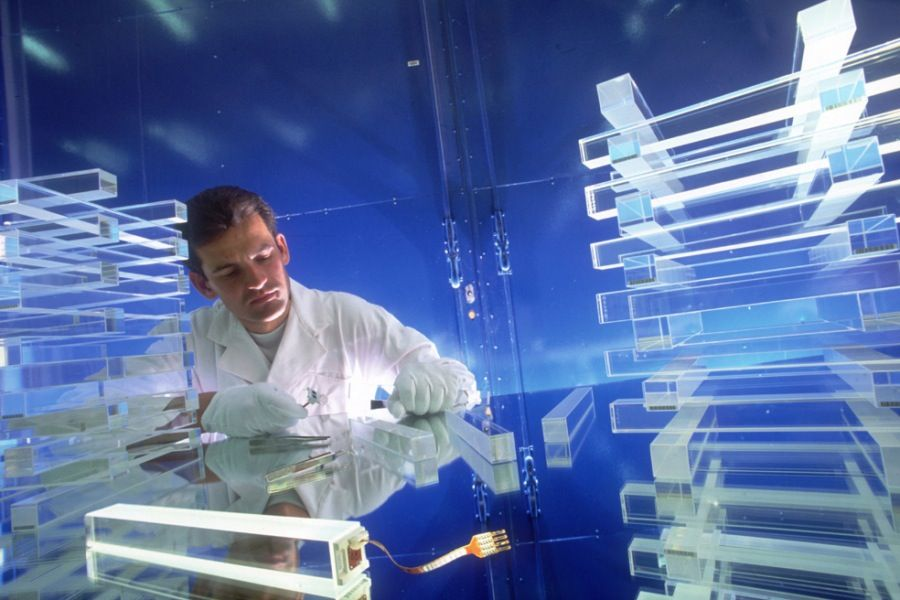
\includegraphics[width=0.49\textwidth,height=10cm,keepaspectratio]{Figures/ECAL_crystals_fancy_lab.jpg}
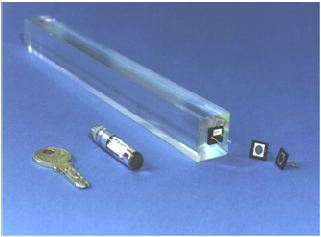
\includegraphics[width=0.49\textwidth,height=10cm,keepaspectratio]{Figures/ECAL_crystal_sizecomparison.jpg}
    \caption{
    (Left) ECAL crystals are grown in a lab.
    (Right) Although made mostly of metal, ECAL crystals are transparent and have a photomultiplier detector attached at the end.} 
    \label{fig:ecal_crystals}
\end{figure}
%%%%%%%%%%%%%%%%%%%%
Electrons and photons interact electromagnetically with the ECAL, creating an electromagnetic (EM) shower, and effectively get trapped here.
The ECAL crystals then give off light (\emph{scintillate}) in proportion to the amount of energy deposited by the electron or photon. 
The scintillator photons are detected by a photomultiplier detector attached to the back of each ECAL crystal (Fig.~\ref{fig:ecal_crystals}, Right).
The ECAL has a barrel component and endcap components.

How does one distinguish between an electron energy deposit in the ECAL system versus and a photon deposit?
The electron will leave hits in the Tracker whereas a photon is electrically neutral and will not generate any signal in the Silicon Tracker. 
So long as the Tracker and ECAL communicate effectively with each other, then they help distinguish between electrons and photons.
Charged hadrons also interact with the ECAL, but only minimally. They very often punch through the ECAL system.
Neutral hadrons can be detected by the ECAL preshower near the ECAL endcaps. 
which helps distinguish a single photon from $\pi^{0}$ mesons as they decay into two photons with a narrow opening angle, making it look as if the two photons are a single photon.

What about those hadrons? They got through the ECAL... To detect hadrons effectively, we need a Hadron Calorimeter.
% That's what we see here with the blue dashed line (the photon) and the red line (the positron).

%%%%%%%%%%%%%%%%%%
%----- HCAL -----%
%%%%%%%%%%%%%%%%%%
\section{Hadron Calorimeter}
By the time particles reach the {\bf Hadron Calorimeter} (HCAL), the only kind which remain (usually) are muons and hadrons.
At 1 meter thick, the HCAL is a brass scintillator and its primary purpose is to catch and record the energies of hadrons.
Similar to the ECAL, the HCAL will scintillate in proportion to the amount of energy of the captured particle. 
The incoming hadrons will \emph{hadronize} (\ie, produce a hadronic shower), generating jets of quarks and gluons which are bound in various ways forming protons, neutrons, pions, kaons, \etc.
Interestingly, the HCAL is made using over a million old, brass shell casings from the Russian Navy back from World War II.
% kinds of particles which have not decayed on their own or were not caught by the ECAL, ,  or when it catches hadronic material: stuff made of quarks, like . 







%%%%%%%%%%%%%%%%%%%%%%%%
%----- MUON SYSTEM-----%
%%%%%%%%%%%%%%%%%%%%%%%%
\section{The Muon System}

The muon detection system is one of the most important systems in CMS, which may seem odd since it is the farthest subdetector from the IP.
The name Compact {\it Muon} Solenoid alludes to its importance.
%  is the {\bf Muon System} and is what puts the {\it Muon} in Compact {\it Muon} Solenoid.
By the time particles make it out to the Muon System, CMS has filtered out nearly everything else: electrons, photons, and hadrons.
The only \emph{detectable} particles remaining at this point are muons, which interestingly will travel way outside of CMS before decaying, upwards of 100s of kilometers before decaying to an electron and neutrino (neutrinos are the only particles which CMS can't explicitly detect).
% We can only assume that we produced neutrinos when momentum is apparently not conserved in an event. 
% When the protons collide at the IP they have nearly zero momentum perpendicular to the beam pipe. 
% This is called transverse momentum, because it's well... transverse to the beam pipe, the z direction.
% If we track, tag, capture all the outgoing particles and reconstruct their transverse momenta, 
% if we find out that it is NOT zero by a large amount, then we say that 

The main purpose of the Muon System is to precisely determine the position and timing of muons.
% \begin{enumerate}
%     \item 
%     % for offline analysis.
%     \item Generate muon trigger primitives for the Level-1 trigger system.
% \end{enumerate}
Similar to the Silicon Tracker, the Muon System doesn't try to capture the muons passing through it;
instead it just tracks their positions. 
% In fact our very own Andrey, Guenakh, and Darin have been instrumental in implementing CSCs. 
% There's also an assembly hall downstairs where CSCs were constructed and tested 
% The  specializes muons. Au contraire; it \textit{specializes} in muon detection. 
% The Compact \textit{Muon} Solenoid would be a pretty hypocritical name if CMS did not detect muons. Au contraire; it \textit{specializes} in muon detection. 
% P
%It would be an ironic name if it did not detect muons well. 
The Muon System is comprised of three kinds of gaseous detectors: 
\begin{enumerate}
    \item {\bf Drift Tubes} (DTs) found in the barrel.
    \item {\bf Resistive Plate Chambers} (RPCs) found in both the barrel and endcap.
    \item {\bf Cathode Strip Chambers} (CSCs) found only in the endcap.
\end{enumerate}
Each of these technologies is constructed differently and was designed with a specific purpose. 
% In Chapter~\ref{ch:CSC}, the inner-workings of the CSCs are explained.

This concludes the overall design and purpose of the subdetectors that make up CMS.
Since I have had hands-on experience working on CSCs, I will discuss the CSC components and how it works in more detail in the subsection below.


\subsection{Let Me See These CSCs}

A cathode strip chambers (CSC) is a gaseous detector which specializes in muon detection. 
{\bf Quick Mention:} The University of Florida has been one of the main contributors to the CSC system and was home to one of the testing and assembly facilities before shipping the CSCs off to CERN.
The CSCs are found only on the endcaps of CMS and each endcap holds 270 CSCs (Fig~\ref{fig:CMS_endcap}). 
%%%%%%%%%%%%%%%%%%%%
\begin{figure}[pbth]
\centering
\includegraphics[width=0.49\textwidth,height=10cm,keepaspectratio]{Figures/CSC_endcap_cutaway.png}
\includegraphics[width=0.49\textwidth,height=10cm,keepaspectratio]{Figures/CSC_endcap_real.png}
    \caption{
    (Left) A cut out view of the ME+ endcap, simulated. Also shown is the coordinate system that CMS uses.
    (Right) The actual ME-2 disk is shown, revealing its ME-2/1 and ME-2/2 rings of CSCs.
    }
    \label{fig:CMS_endcap}
\end{figure}
%%%%%%%%%%%%%%%%%%%%
Each CSC cost about \$100,000 to make, so very quickly this becomes an expensive project.
They are trapezoidal in shape and are composed of 6 layers filled with gas.
The gas surrounds wires and strips which are put under 3,600 V to aid in muon detection as explained below (Fig.~\ref{fig:CSC_guts}). 
%%%%%%%%%%%%%%%%%%%%
\begin{figure}[pbth]
\centering
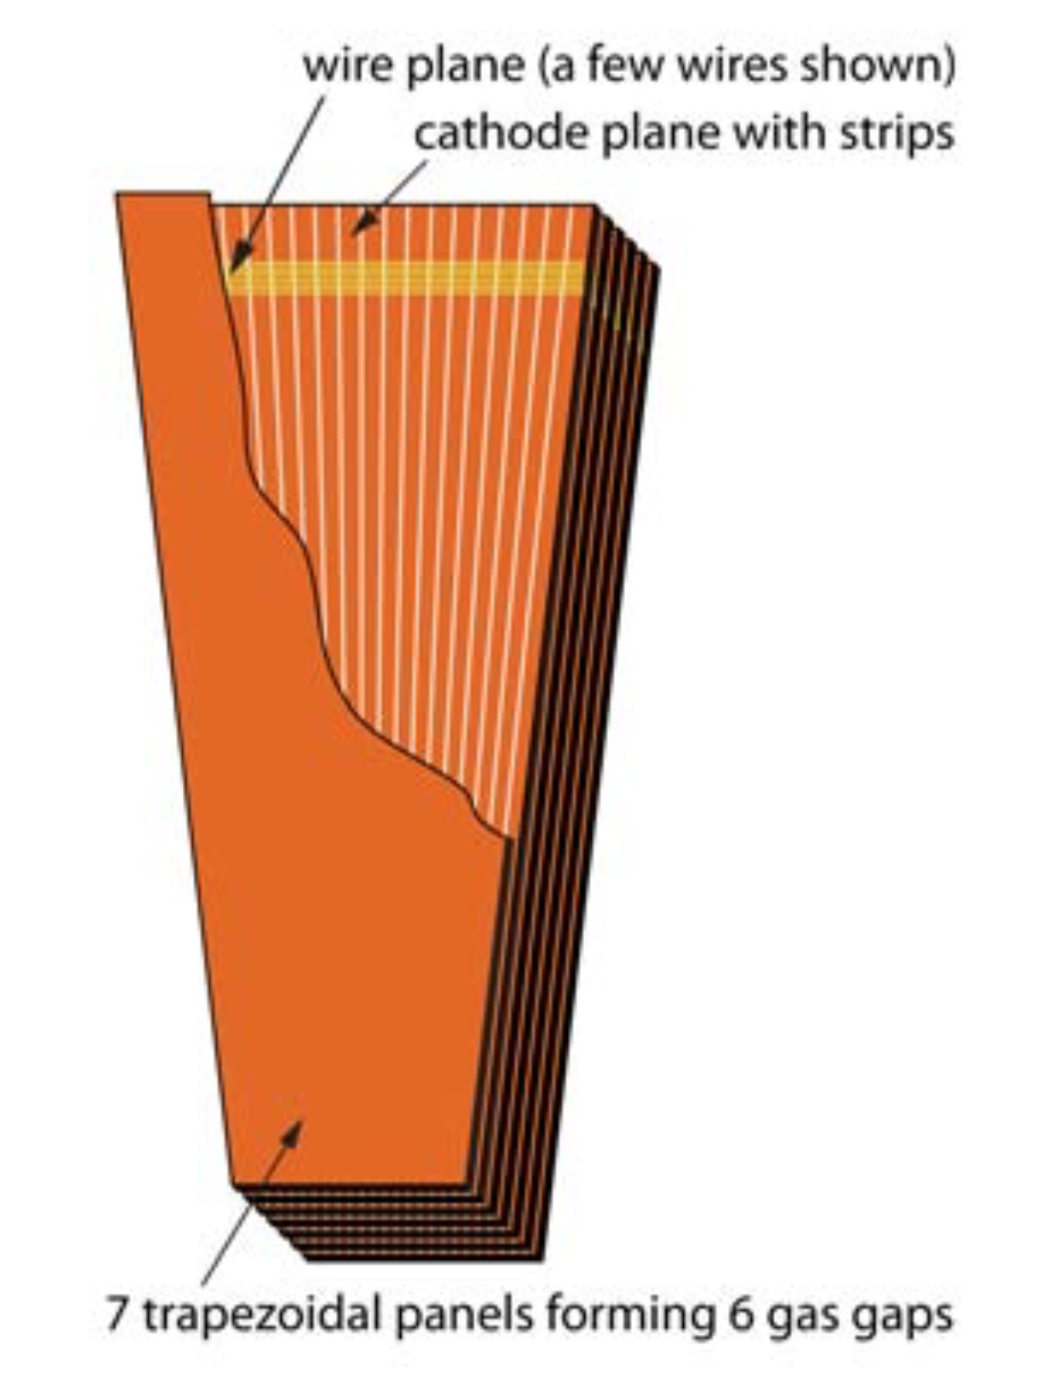
\includegraphics[width=0.49\textwidth,height=10cm,keepaspectratio]{Figures/CSC_cutaway_view_new.png}
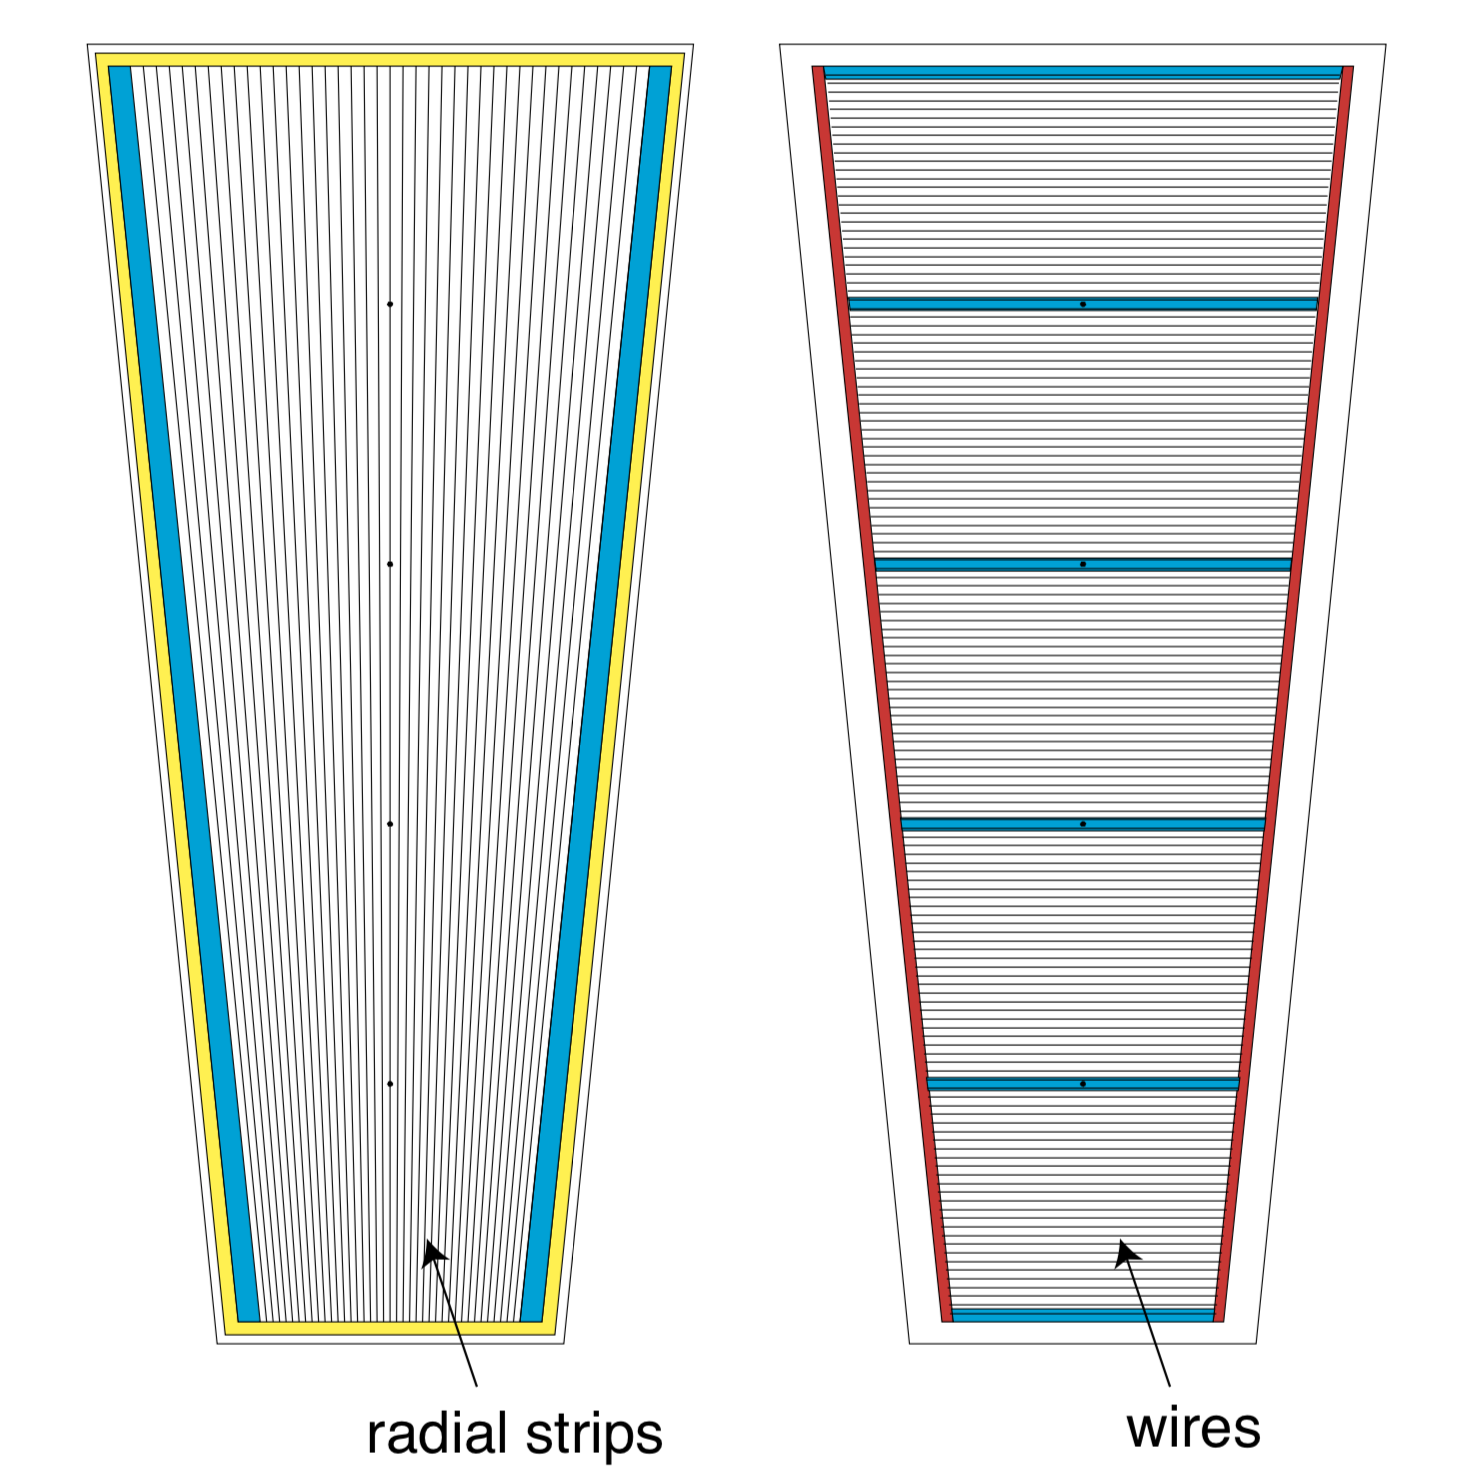
\includegraphics[width=0.49\textwidth,height=10cm,keepaspectratio]{Figures/CSC_stripsandwires.png}
    \caption{
    (Left) A CSC with its top layer exposed. You can see very thin gold-plated tungsten wires which actually span the entire width of the CSC. 
    Thicker vertical strips run along the length.
    (Right) More detail showing the radial strips and the horizontal wires. Also shown is the 5 segments of a CSC.
    }
    \label{fig:CSC_guts}
\end{figure}
%%%%%%%%%%%%%%%%%%%%
The gaseous mixture of ${\rm Ar:CO_{2}:CF_{4} }$ in the ratio of $5:4:1$ has been specially designed to maximize the lifetime of the CSC as it endures radiation damage over the years. 
In each layer, the gas mixture surrounds approximately 80 copper strips, each about 1 cm wide that span radially away from the IP.
Also inside the layers are over 1,000 gold-plated tungsten wires, which run azimuthally in the CMS coordinate system.
When the strips and wires detect muons they provide an (x,y) coordinate system to track the muon. 
As the muon passes through the remaining layers of the CSC, this provides a z coordinate as well, giving the Muon System the ability to ``see'' the full muon trajectory.
% In conjunction with the Silicon Tracker measurements, muon momentum can be measured to a precision of 

{\bf Labelling the CSCs:} 
The two endcaps are labelled as ``ME+'' and ``ME-'', depending on in which z-direction they sit. 
Since they are structurally the same, let's focus on the ME+ endcap for a moment. 
The ME+ endcap has four disks, where ME+1 is the first disk, the one closest to the IP, and ME+4 is the fourth and farthest away. 
Similarly for the ME$-$ endcap. 
Then, within each disk, there are either two or three ``rings'' of CSCs, as shown in Fig~\ref{fig:CMS_long_view_subdetectors} (green).
These rings are labelled like ME+2/1, which would indicate the second disk and the first (innermost) ring, radially closest to the IP.
All rings contain 36 CSCs, except for ME${\rm \pm X}$/1, for $\x=$ 2,3,4, which contain only 18 CSCs.
Finally, the CSCs are given one, last number to label them on the ring:
the CSC that sits along the positive x-axis in CMS's coordinate system is given the number ``01'', \eg\ ME+4/2/01. 
The CSCs are then incrementally numbered as you go around in a positive azimuthal direction.
%%%%%%%%%%%%%%%%%%%%
\begin{figure}[pbth]
\centering
\includegraphics[width=15cm,height=10cm,keepaspectratio]{Figures/CMS_longitudinal_view.png}
    \caption{
    Longitudinal cross section of CMS, showing the different pseudorapidity values ($\eta$) and also the different subdetector regions.
    }
    \label{fig:CMS_long_view_subdetectors}
\end{figure}
%%%%%%%%%%%%%%%%%%%%

{\bf Detecting Muons:}
When a muon passes through a layer of a CSC, it has the chance to ionize an Ar atom (Fig.~\ref{fig:e_avalanche}).
Since the wires are under high voltage (3,600 V), the ionized electron accelerates towards the positively-charged wire, and in doing so it ionizes many Ar atoms which are along its path. 
Starting from just a single electron, the multiplicity can go as high as 100,000 ionized electrons, thereby creating what is known as an electron avalanche. 
This phenomenon is called ``gas gain''.
%%%%%%%%%%%%%%%%%%%%
\begin{figure}[pbth]
\centering
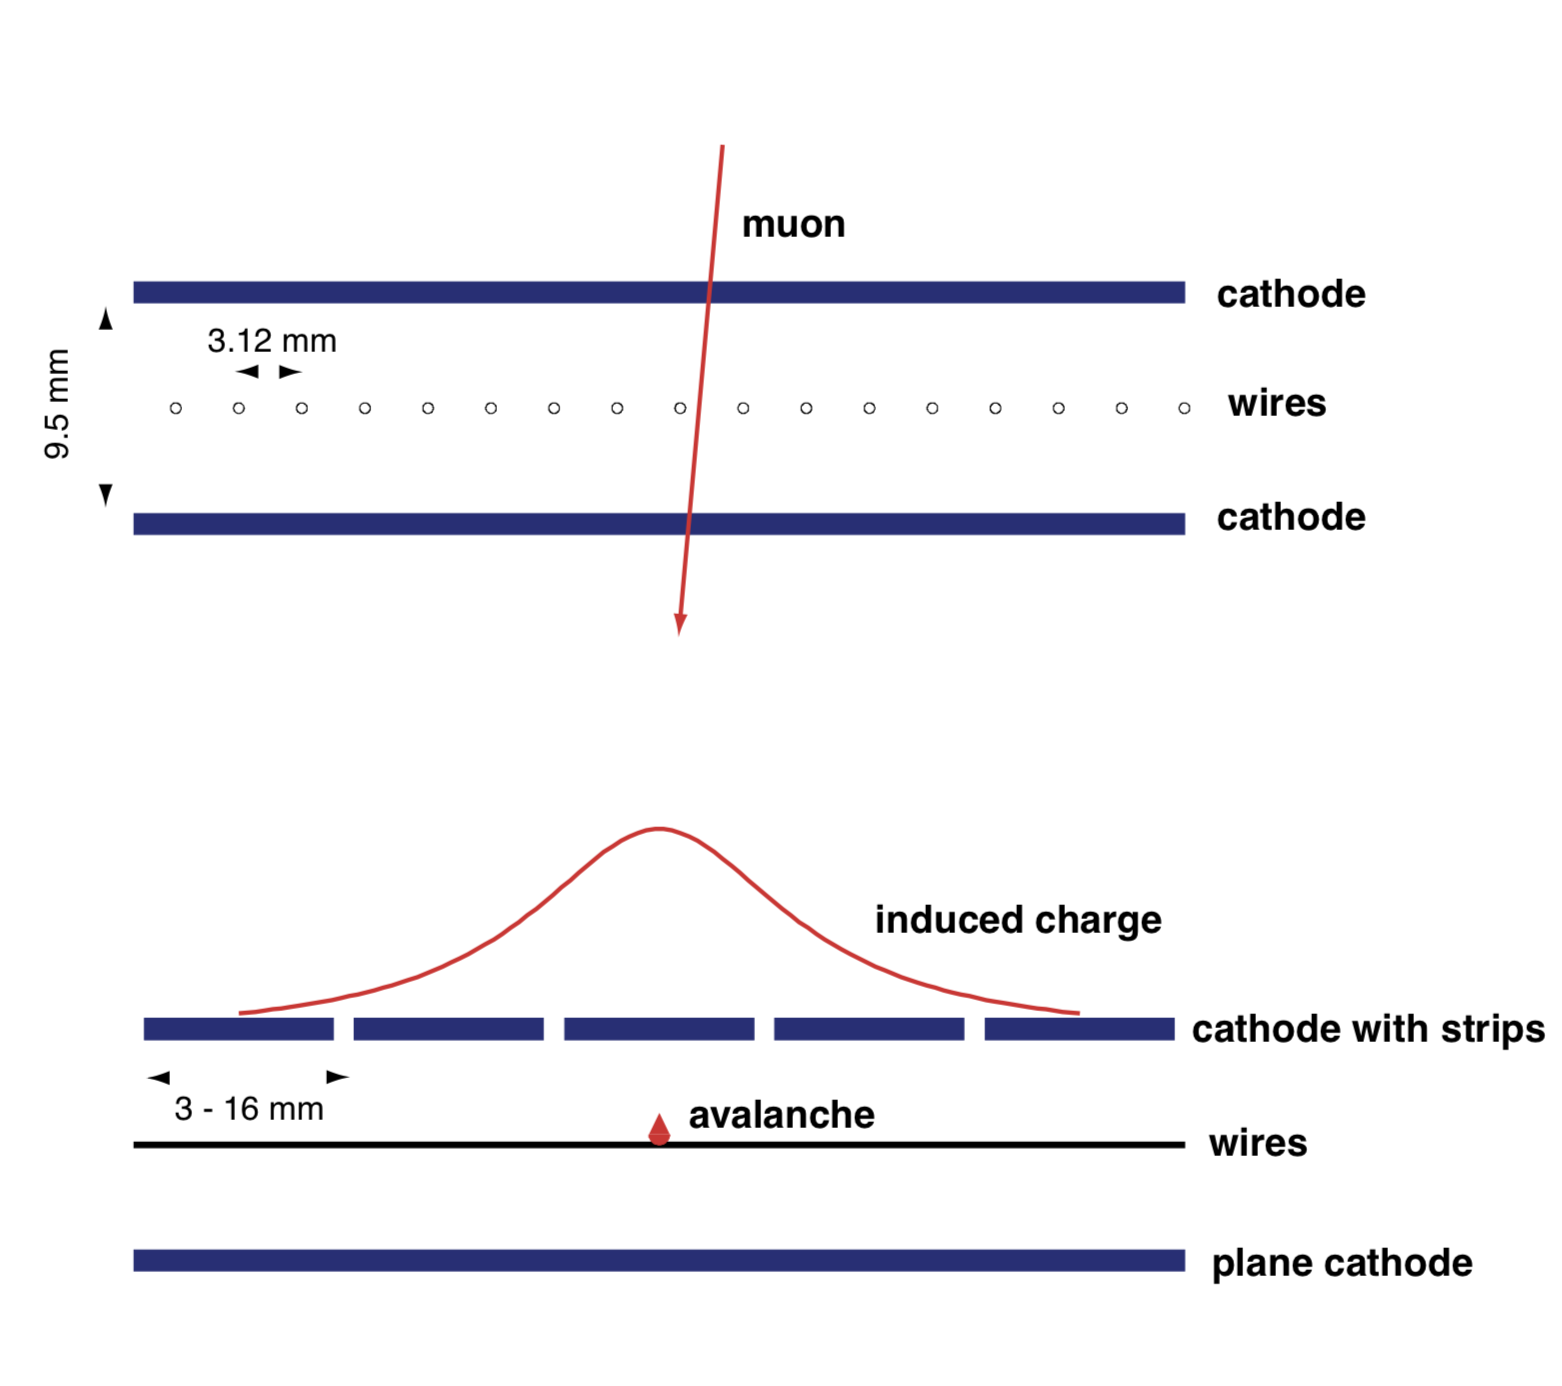
\includegraphics[width=15cm,height=10cm,keepaspectratio]{Figures/CSC_elec_avalanche_old.png}
    \caption{
    A muon passes through one of the gaseous layers of the CSC, ionizing the gas mixture and inducing a charge on the wires and strips. 
    }
    \label{fig:e_avalanche}
\end{figure}
%%%%%%%%%%%%%%%%%%%%
The electrons travel onto the wire and become an electrical signal which then gets sent to the anode front-end boards (AFEBs) for further signal processing.
The ionized Ar$^+$ will similarly distribute a charge signal on the negative strips. 
This cluster of charge is much more widely spread over the strips compared to the charge on the wires.
Therefore, comparator logic is implemented to narrow down the precision to the order of 100 $\mu$m by using half-strip information (Fig.~\ref{fig:comparators}).
%%%%%%%%%%%%%%%%%%%%
\begin{figure}[pbth]
\centering
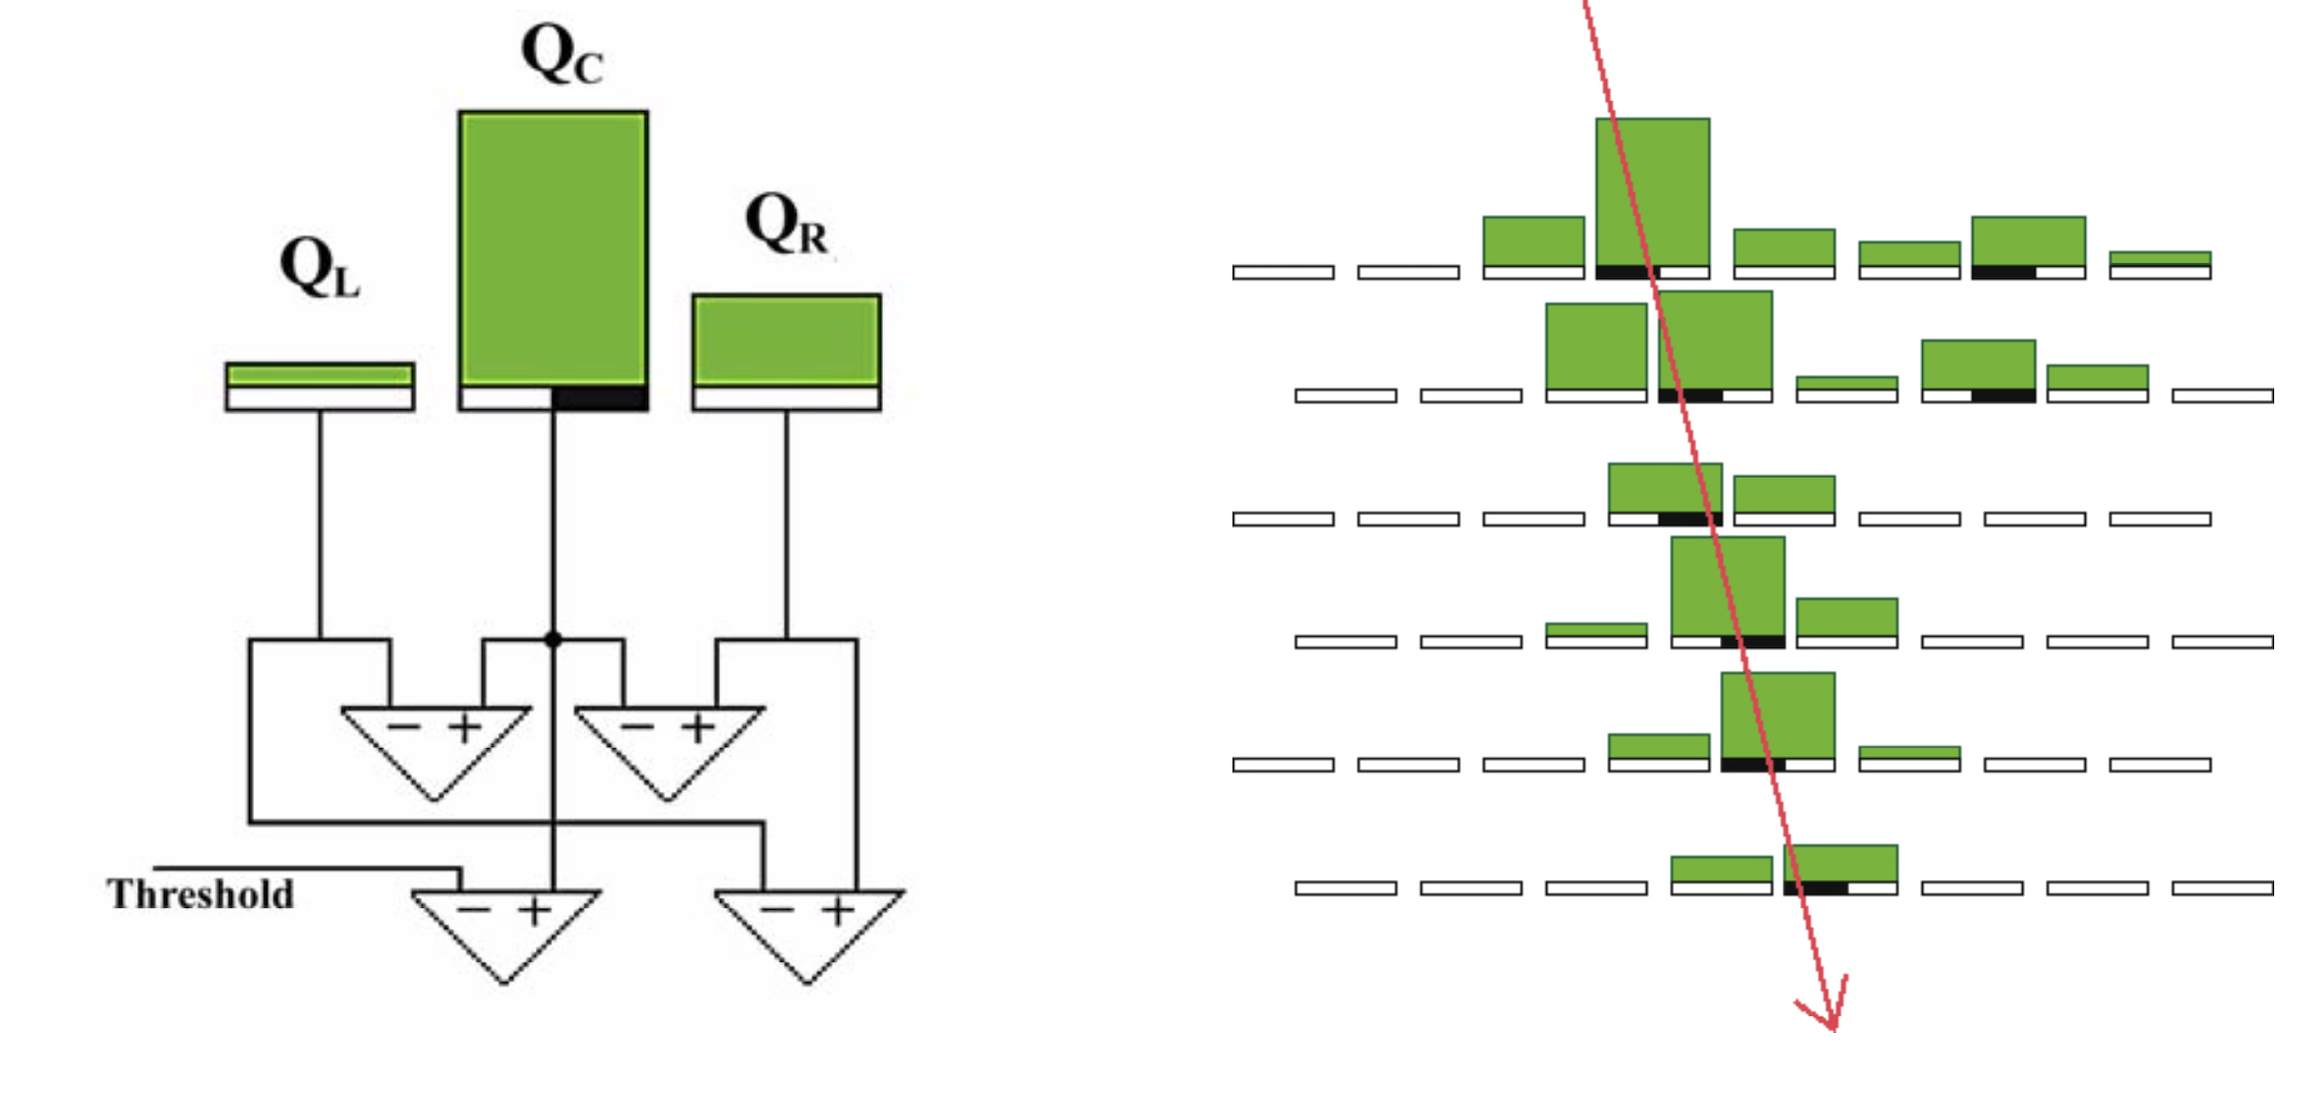
\includegraphics[width=15cm,height=10cm,keepaspectratio]{Figures/CSC_comparators_and_strips.png}
    \caption{
    (Left) Comparators are used to compare neighboring strip cluster charge to determine on which half-strip the peak charge resided.
    (Right) A muon passes through all six layers of a CSC inducing charge on various half-strips.
    % cathode front-end board (CFEB) 
    }
    \label{fig:comparators}
\end{figure}
%%%%%%%%%%%%%%%%%%%%

The muon will continue passing through the next 5 layers, repeating the process of ionizing the gas mixture, and depositing an electrical signal on the wires. 
he wires and strips provide (x,y)-coordinates, and as the muon passes through the CSC, the other layers provide a z-coordinate, revealing the path of the muon.
% The AFEBs then digitize this analog signal using ADCs and 
Depending on how many hits were recorded by the CSC will determine if a muon event was significant enough to be registered as a real muon. 
If so, then its precise positions on the wires and strips will be read out by the Data Acquisition (DAQ) system and be stored for further data analysis.

% \subsection{Drift Tubes}
% \subsection{Resistive Plate Chambers}

% \subsection{Endcap Muon Electronics}
% In order to conclude that a muon definitely passed by the muon detectors, a very sophisticated electronics system has been developed. 

% Hmm... EMU is just for the endcaps. This system is called "EMU" and 

% I had been working on CMS analyses for about a year and a half before I actually saw CMS just earlier this year. And let me tell you: It is HUGE! 
% Next I am going to elaborate more on the CSCs, since my first experience with CMS hands-on work with CSCs. 

% The muon barrel system, after it talks with the tracker system, has a muon pT resolution of 1.5% in the barrel and ~6% in the endcap.

% Trigger system:
% Since the event  rate and data rate are so high, and most of the events are uninteresting, typical physics,
% we need a fast-working filtration system to sift through the good and bad events. 
% We want to "trigger" on the good events but only have about 4 μs to do so. 
% This is the job of the L1 trigger and and the High-Level Trigger. 
% I'm not going to explain any more of this because it is an extremely sophisticated system. 